\documentclass[10pt]{beamer}

\usetheme[progressbar=frametitle]{metropolis}
\usepackage{appendixnumberbeamer}

\usepackage{booktabs}
\usepackage[scale=2]{ccicons}

\usepackage{pgfplots}
\usepgfplotslibrary{dateplot}

\usepackage{movie15}

\usepackage{xspace}
\newcommand{\themename}{\textbf{\textsc{metropolis}}\xspace}
\newcommand\nd{\textsuperscript{nd}\xspace}
\newcommand\rd{\textsuperscript{rd}\xspace}
\newcommand\nth{\textsuperscript{th}\xspace}

\usepackage{amsthm}
\usepackage{lineno}
\usepackage{amssymb,graphics,color,cite,amsmath}
\usepackage{wrapfig}

\usepackage{media9}%


\title{Mathematical Models for Red Blood Cell}
\subtitle{2018 Summer AM-SURE}
\date{}
\author{Tianrui Xu, advised by Charles S. Peskin}
% tx392@nyu.edu}
\institute{Courant Institute of Mathematical Sciences, New York University}

\begin{document}

\maketitle

\begin{frame}[fragile]{Red Blood Cell}
%Say about my motivation: the importance of membrane and how I become interested in this topic
\begin{figure}[h]
	\centering
	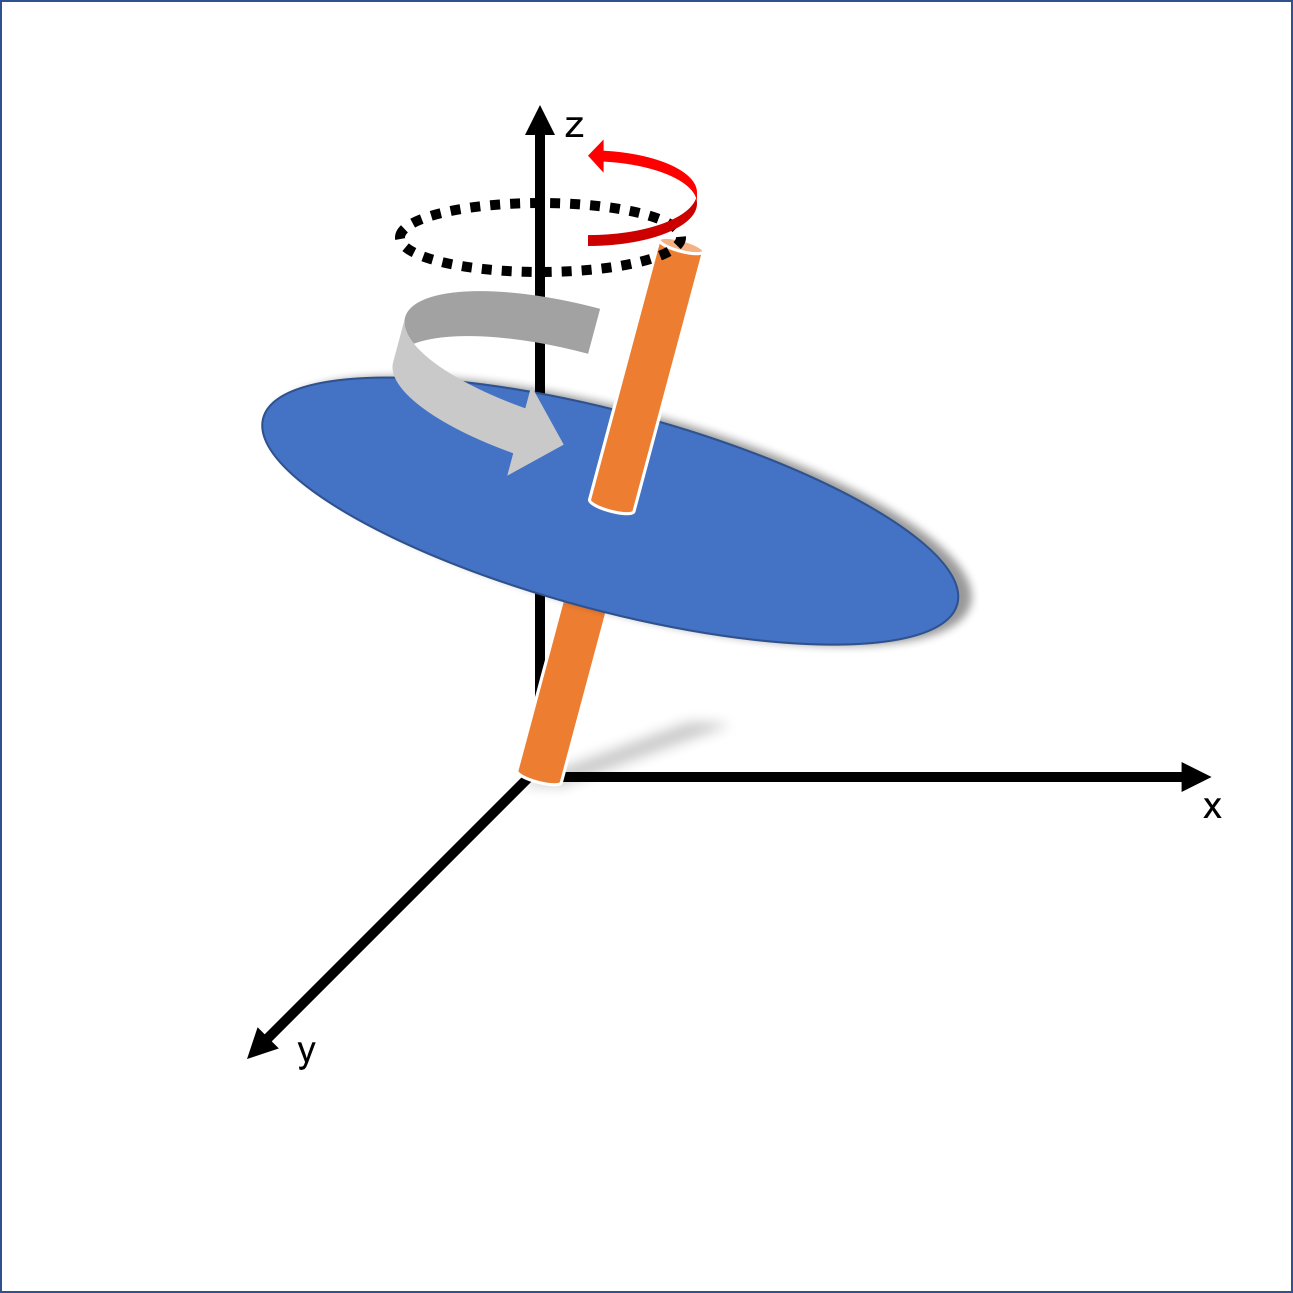
\includegraphics[width=0.6\textwidth]{sphere1.png}
%%	\caption{Red Blood Cell}\label{Fig:RBC}
\end{figure}

\end{frame}

\begin{frame}{Goal}
%This special shape motivates us to build a model for the red blood cell to show how it starts from a random shape and eventually becomes biconcave. Although there are many past studies on models of red blood cell, the goal of this project is to

Find the most \underline{simplest} equation and use \underline{discrete} methods to generate a \underline{biconcave} shape from a perfect sphere.

\end{frame}

\section{Mathematical Modeling}

\begin{frame}{Triangulated Surface}
%The discrete method we use to model a sphere, is triangulated surface. We divide the surface into as many flat triangles as possible and the more triangles we use, the more smooth the surface is \cite{sphere} (see figures 1(a) and (b)). By triangulating the surface, we are able to track the coordinates of every points which are vertices of triangles. To force the membrane to change, we can simply force every points (vertices) to move and then the surface will follow.

We start from a sphere (codes from Professor Peskin).

\begin{figure}[h]
	\begin{minipage}{0.48\textwidth}
		\centering
		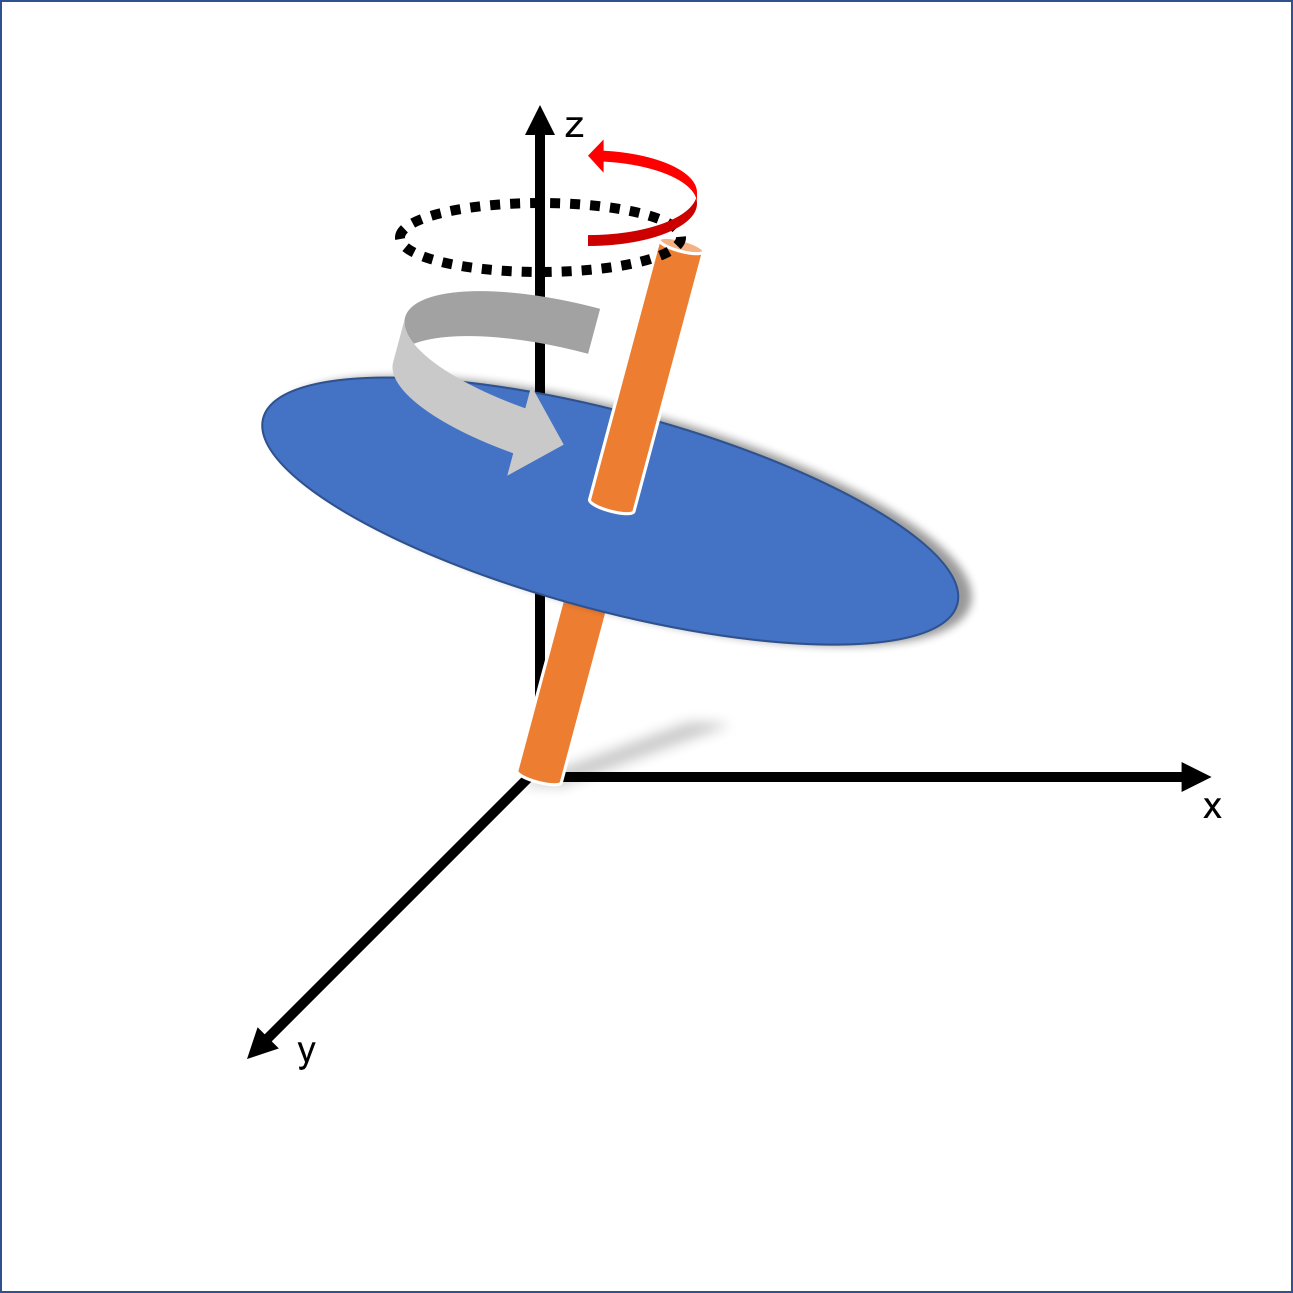
\includegraphics[width=0.86\textwidth]{sphere1.png}
	\end{minipage}
	\begin{minipage}{0.48\textwidth}
		\centering
		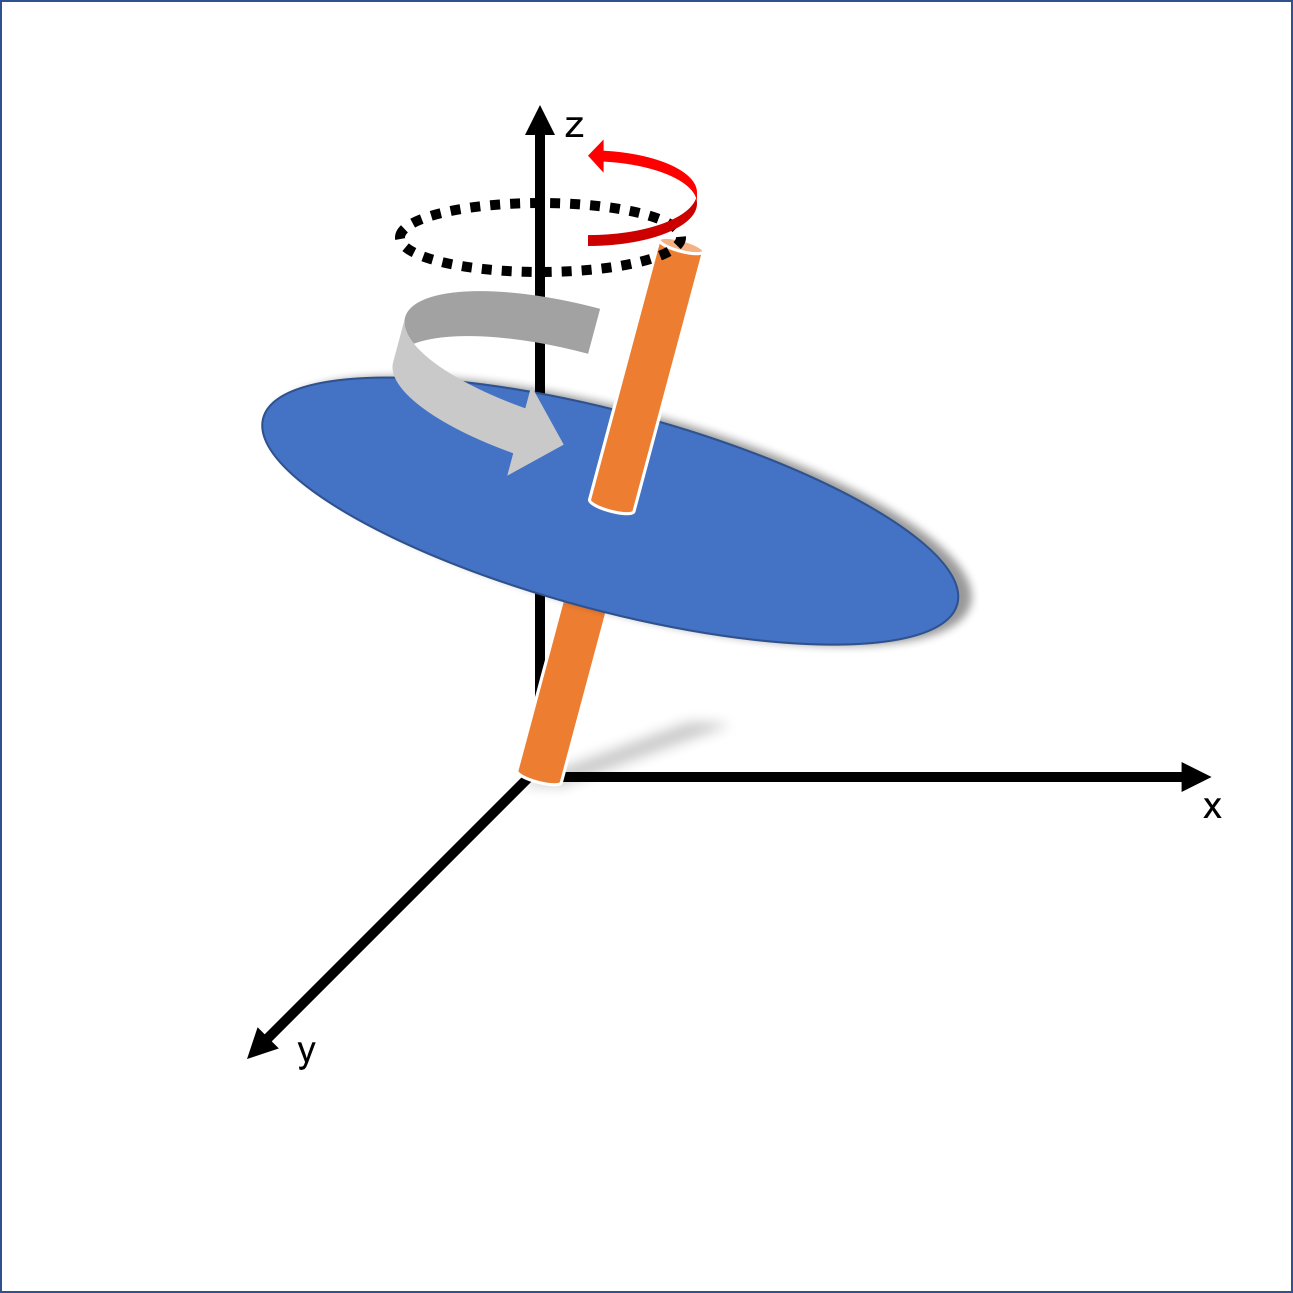
\includegraphics[width=0.9\textwidth]{sphere1.png}
	\end{minipage}
\end{figure}

The more triangles we use, the more smooth the surface is.
\end{frame}

\begin{frame}{Model Setup}

%The reason why a red blood cell is in a biconcave shape, instead of any other shapes, is that the biconcave shape requires the least amount of bending energy. If we allow the membrane of a cell to move freely, it will eventually bend to the biconcave shape to minimize its membrane's bending energy. Therefore, to obtain the shape of a red blood cell, we first minimize the bending energy $E$.

Discovered by Canham in 1970, the biconcave shape requires the least amount of bending energy $E$.
\begin{itemize}
\item Minimize $E$.
%find a path
\item Minimize $\frac{dE}{dt}$, where $t$ refers to time.
%then we can find a direction that decreases $E$ in the fastest speed. This leads us to minimize $\frac{dE}{dt}$, where $t$ refers to time.

%If there is no bound on the speed at which $E$ can decrease, we can always find a faster speed by making some points moving faster and making the shape of our membrane changing faster. To achieve a balance between the speed of $E$ and the speed of points on our surface, we would like to add a cost when energy decreases faster and this cost is the speed of points.
\item Minimize $\frac{dE}{dt} +\frac{1}{2}\sum_{k} \frac{dX_{k}}{dt} \frac{dX_{k}}{dt}$, where $X_{k}$ is the coordinate vector of the $k\nth$ point.
\end{itemize}

\end{frame}

\begin{frame}{Constraints}

\begin{itemize}

\item Area: Surface area should remain constant: $\frac{dA}{dt} = 0$.

\vspace{5mm}

\item Volume: Force the volume to decrease: $\frac{dV}{dt} = \frac{dV_{0}}{dt}$

\end{itemize}

\end{frame}

\begin{frame}{Constraints}

$V_{0}(t) = V\min + (V\max-V\min)e^{-at}$, where $V_{max}$ refers to the initial volume, $V_{min}$ refers to the final volume, and $a$ is a positive constant.

\begin{figure}
	\centering
	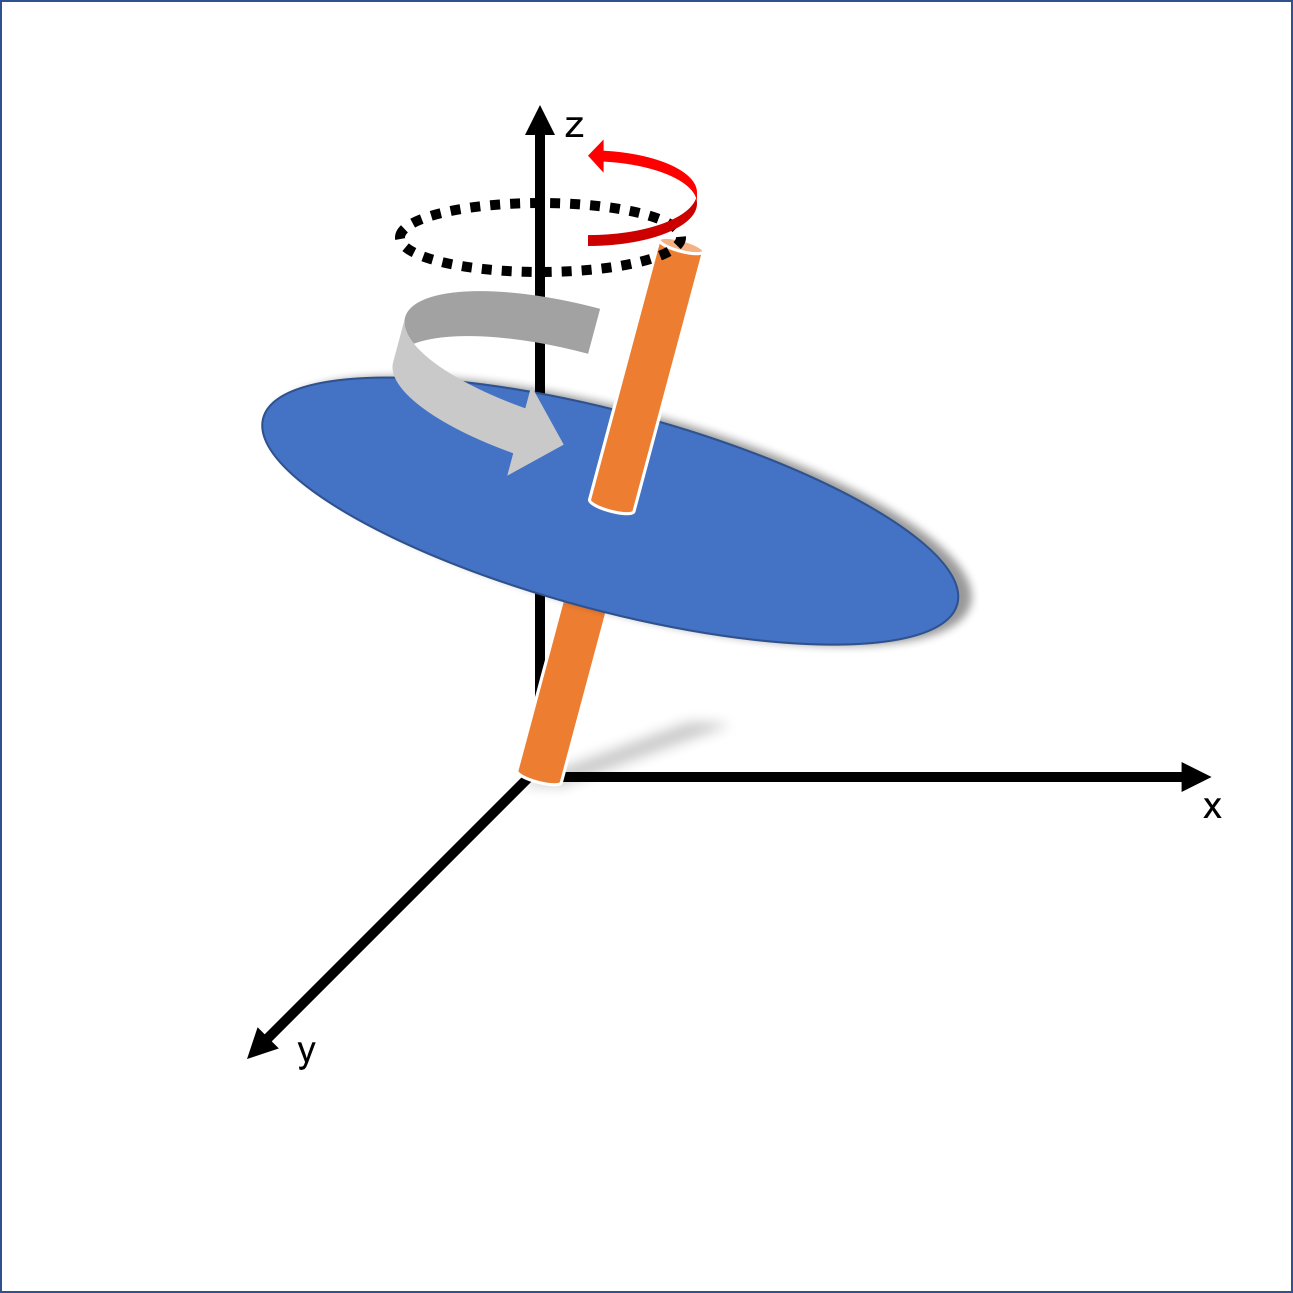
\includegraphics[width=0.8\textwidth]{sphere1.png}
\end{figure}

%Given a surface area fixed, the shape with the largest volume is a sphere. However, since we start from a sphere and want to keep surface area constant, we have to force volume $V$ to decrease, to ensure possible movements of points in our model.
\end{frame}


\begin{frame}
\begin{itemize}
\item In summary:

\small
\begin{equation}
\text{Minimize} \quad \frac{dE}{dt} +\frac{1}{2}\sum_{k} \frac{dX_{k}}{dt} \frac{dX_{k}}{dt},\quad \text{subject to}\quad \frac{dV}{dt} = \frac{dV_{0}}{dt} \quad \text{and}\quad \frac{dA}{dt} = 0. \nonumber
\end{equation}
\normalsize
\vspace{5mm}

\item Translate the above equation into the following ODE equation:
\small
\begin{equation}
\frac{dX_{k}}{dt} = - \frac{\partial E}{\partial X_{k}} - \lambda \frac{\partial V}{\partial X_{k}} - \mu \frac{\partial A}{\partial X_{k}},\quad \text{subject to}\quad \frac{dV}{dt} = \frac{dV_{0}}{dt} \quad \text{and} \quad \frac{dA}{dt} = 0, \nonumber
\end{equation}
\normalsize
where $\lambda$ and $\mu$ are lagrange multipliers for the constraints.

\end{itemize}

\end{frame}

\begin{frame}{Calculation}


\begin{figure}
	\begin{minipage}{0.48\textwidth}
		\centering
		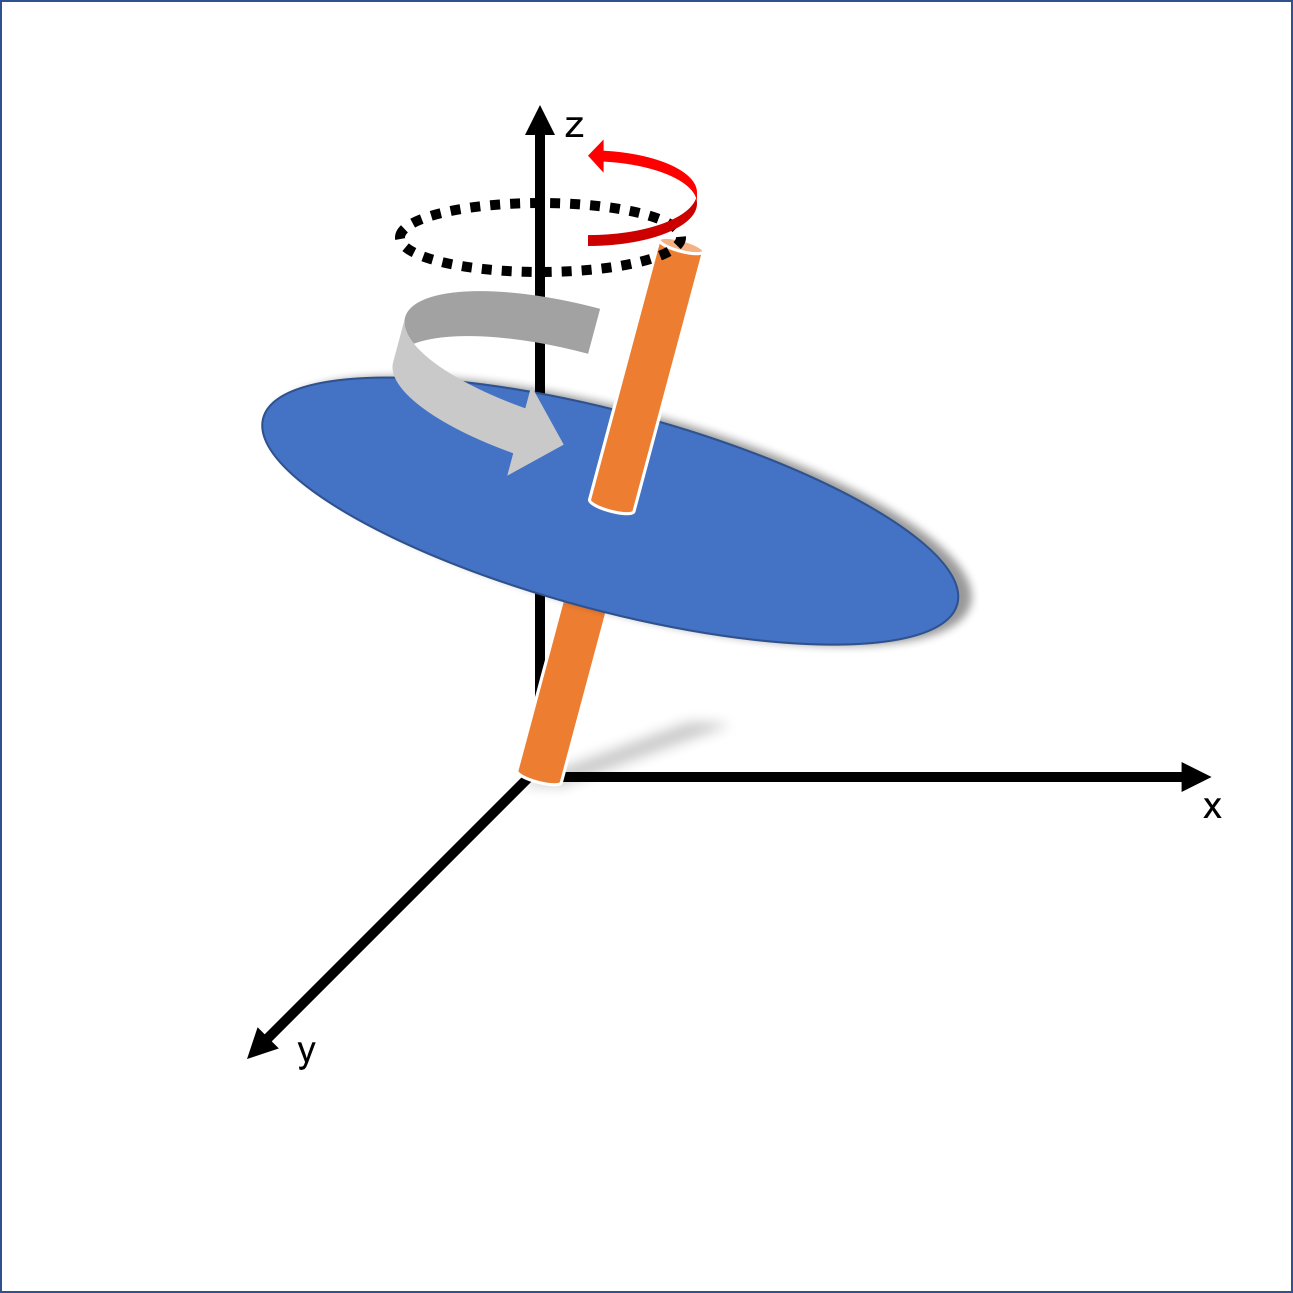
\includegraphics[width=1.05\textwidth]{sphere1.png}
	\end{minipage}
	\begin{minipage}{0.48\textwidth}
		\centering
		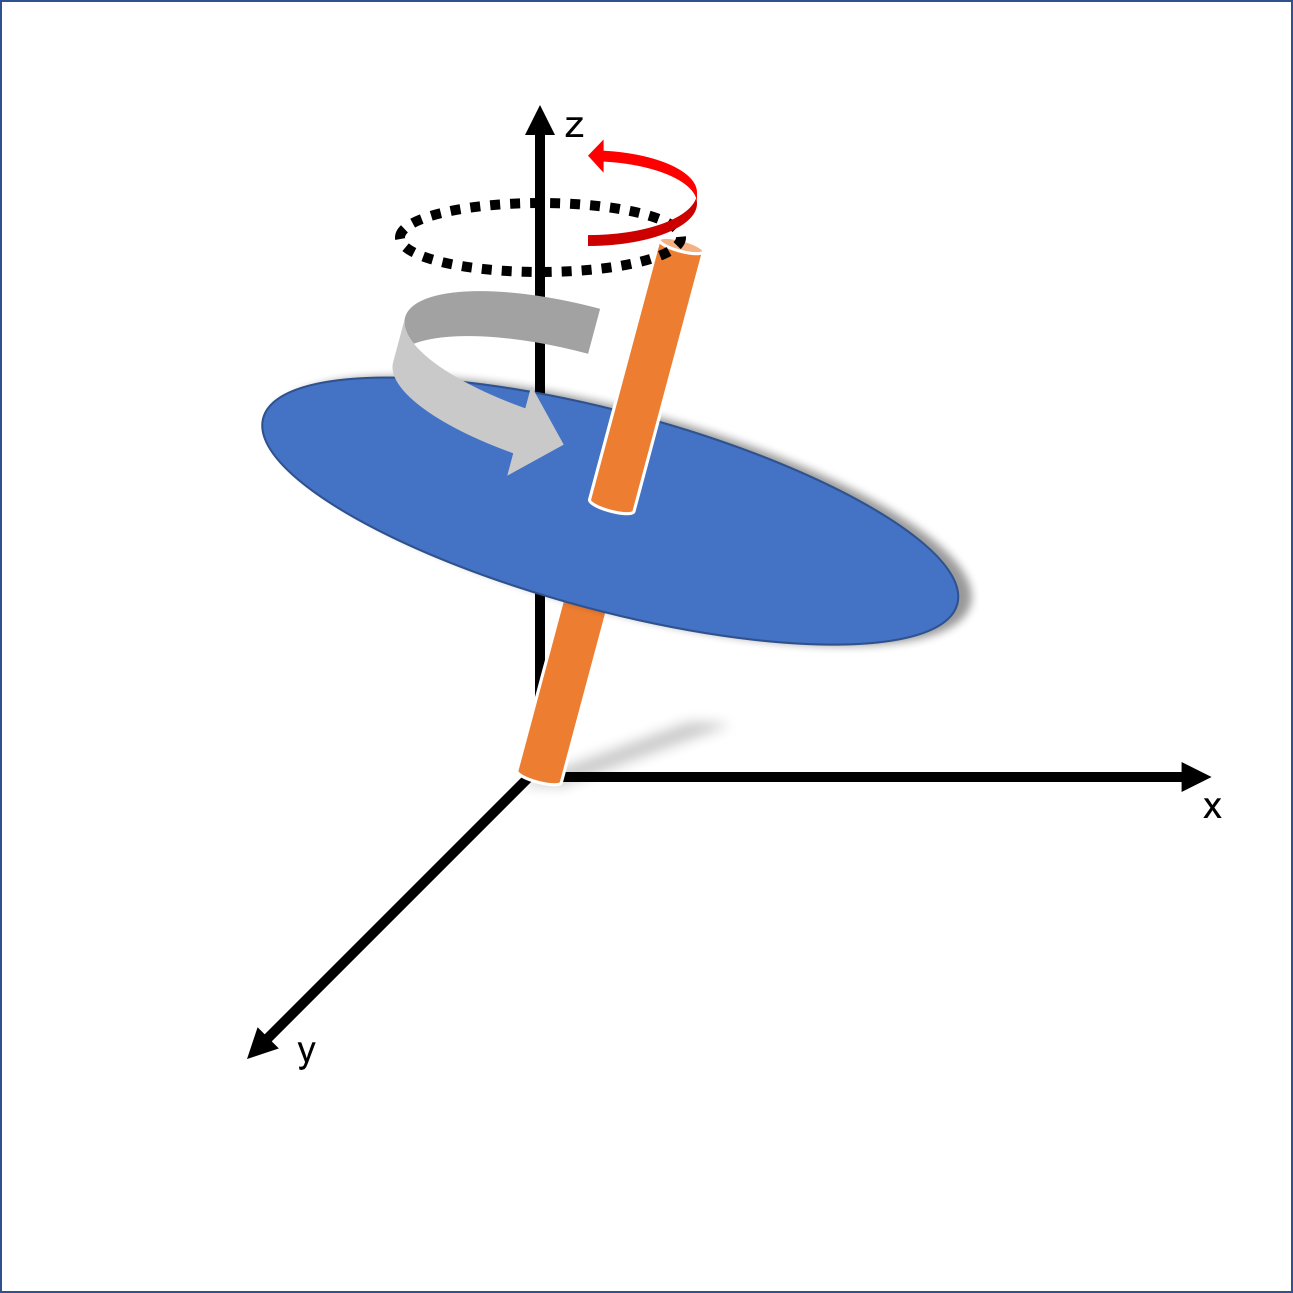
\includegraphics[width=0.93\textwidth]{sphere1.png}
	\end{minipage}
\end{figure}

\end{frame}


\begin{frame}{Calculation}
\begin{wrapfigure}{R}{0.6\textwidth}
	\vspace{-24pt}
	\centering
	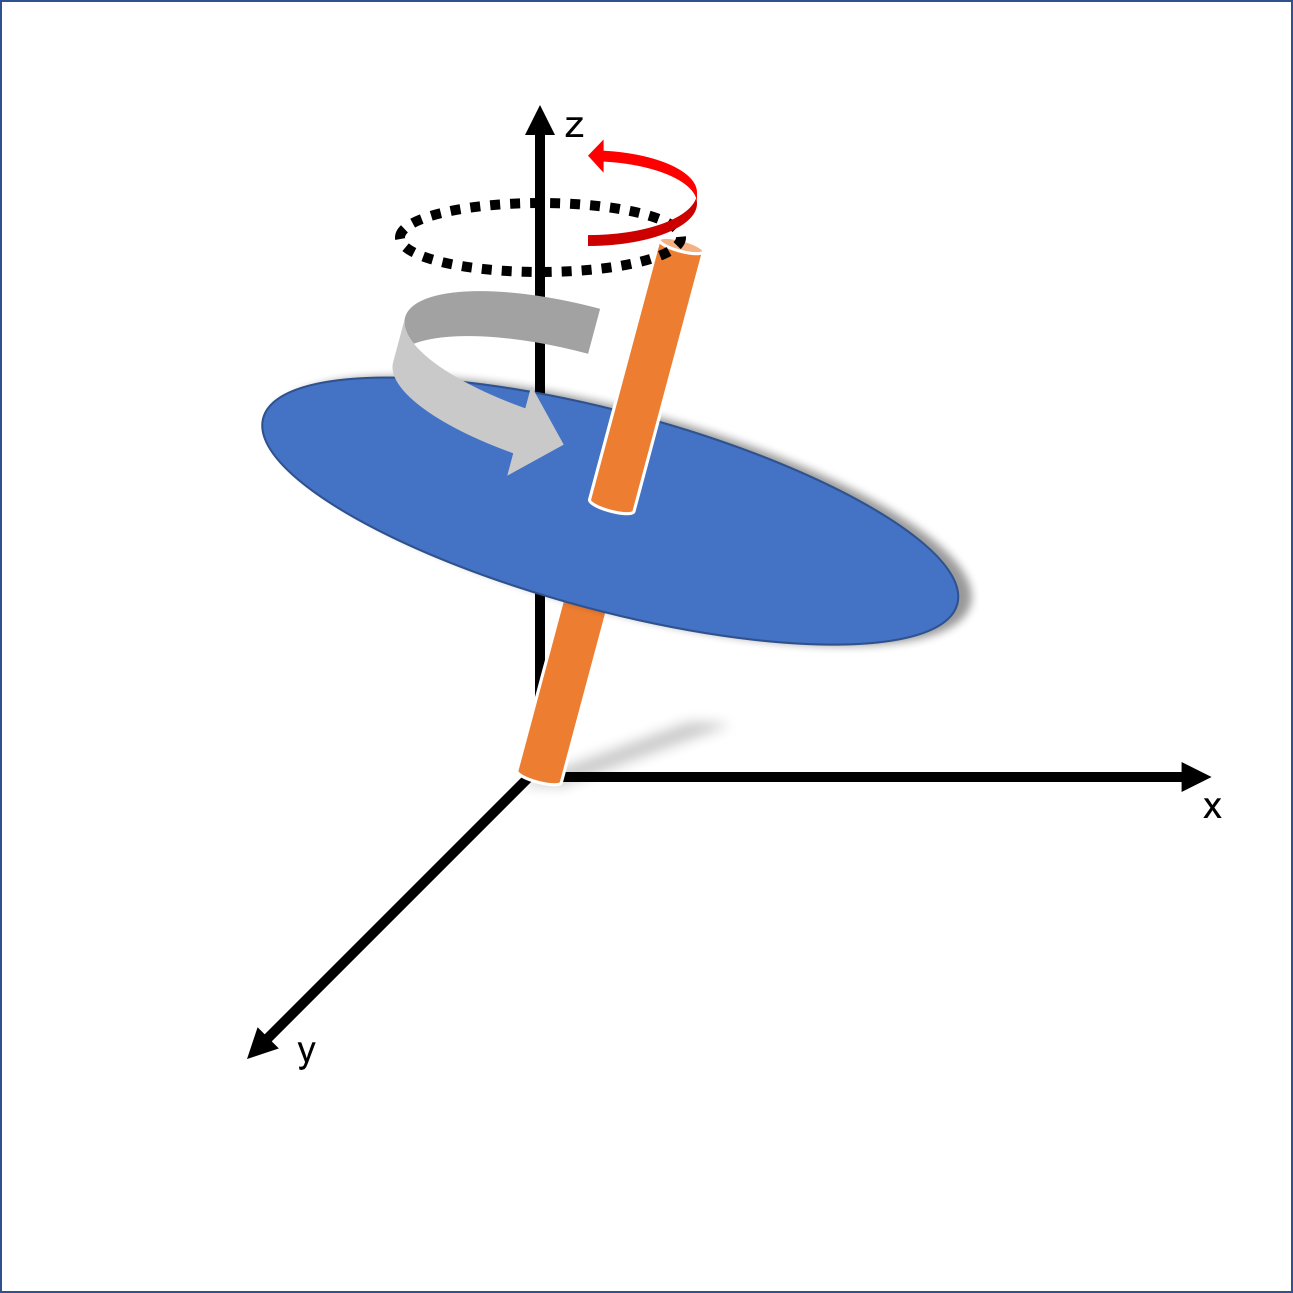
\includegraphics[width=0.5\textwidth]{sphere1.png}
\end{wrapfigure}
Volume $V = \sum_{f} V_{f} $, where $V_{f} = \frac{1}{6} X_{f_1} (X_{f_2} \times X_{f_3})$.

\vspace{5mm}

Surface area $A =  \sum_{f} a_{f}$, where $a_{f} =  [\frac{1}{2}(X_{f_2}-X_{f_1}) \times (X_{f_3}-X_{f_1})] \cdot n$, where $n$ is the normal vector to the surface $f$.
%where V is the sum of volumes of all tetrahedrons. Explain that X_{f_1}, X_{f_2}, X_{f_3} are coordinate vectors.
%$A$ is the sum of areas of all triangles, and $a_{f}$ represents the area of the $f_{th}$ face (triangle). Heron's formula $a_{f}$


%way to calculate $\lambda$ and $\mu$ are not given. if has to say, say the way to calculate \lambda and \mu is very interesting and it is also a wrap up of the whole model and a recap
\end{frame}


\begin{frame}{Calculation}
%we would like to show how to calculate the bending energy $E$, the volume $V$, the surface area $A$, $\lambda$ and $\mu$.

On a smooth surface:\\
(1) Bending energy $E = \int H^2 da$, where $H$ and $a$ represent mean curvature and area, respectively.

(2) Mean curvature $H$ of a surface is the rate of change of its area, per unit area, when this surface is moving in the normal direction to itself.
%Therefore, we would like to apply this definition on our discrete surface

\vspace{5mm}

On discrete surface (face $f$) :\\
(1) Mean curvature $h_{f}$ is the rate of change of face $f$'s area, to its area, when face $f$ is moving in the normal direction to itself.

(2) $h_{f} = (da_{f}/dt)\cdot a_{f}^{-1}$, where $a_{f}$ is the area of the face $f$.

(3) Then $E = \int H^2 da \approx \sum_{f} h_{f}^2a_{f}$.
\end{frame}

\begin{frame}{Non-Smoothness}
%Since we are using a discrete method to approach a continuous problem, it becomes important to keep the surface smooth. Smoothness is important to our model, not only because irregular surface can produce errors, but also because a cell resists too much local change to its membrane. Therefore, to restrict random moments of points in our model, we want to add more constraints or penalties to our ODE equation. One method is to restrict the deformation of triangles, and to achieve this, we should avoid too much change on each triangle edge. I

\begin{figure}[h]
	\centering
	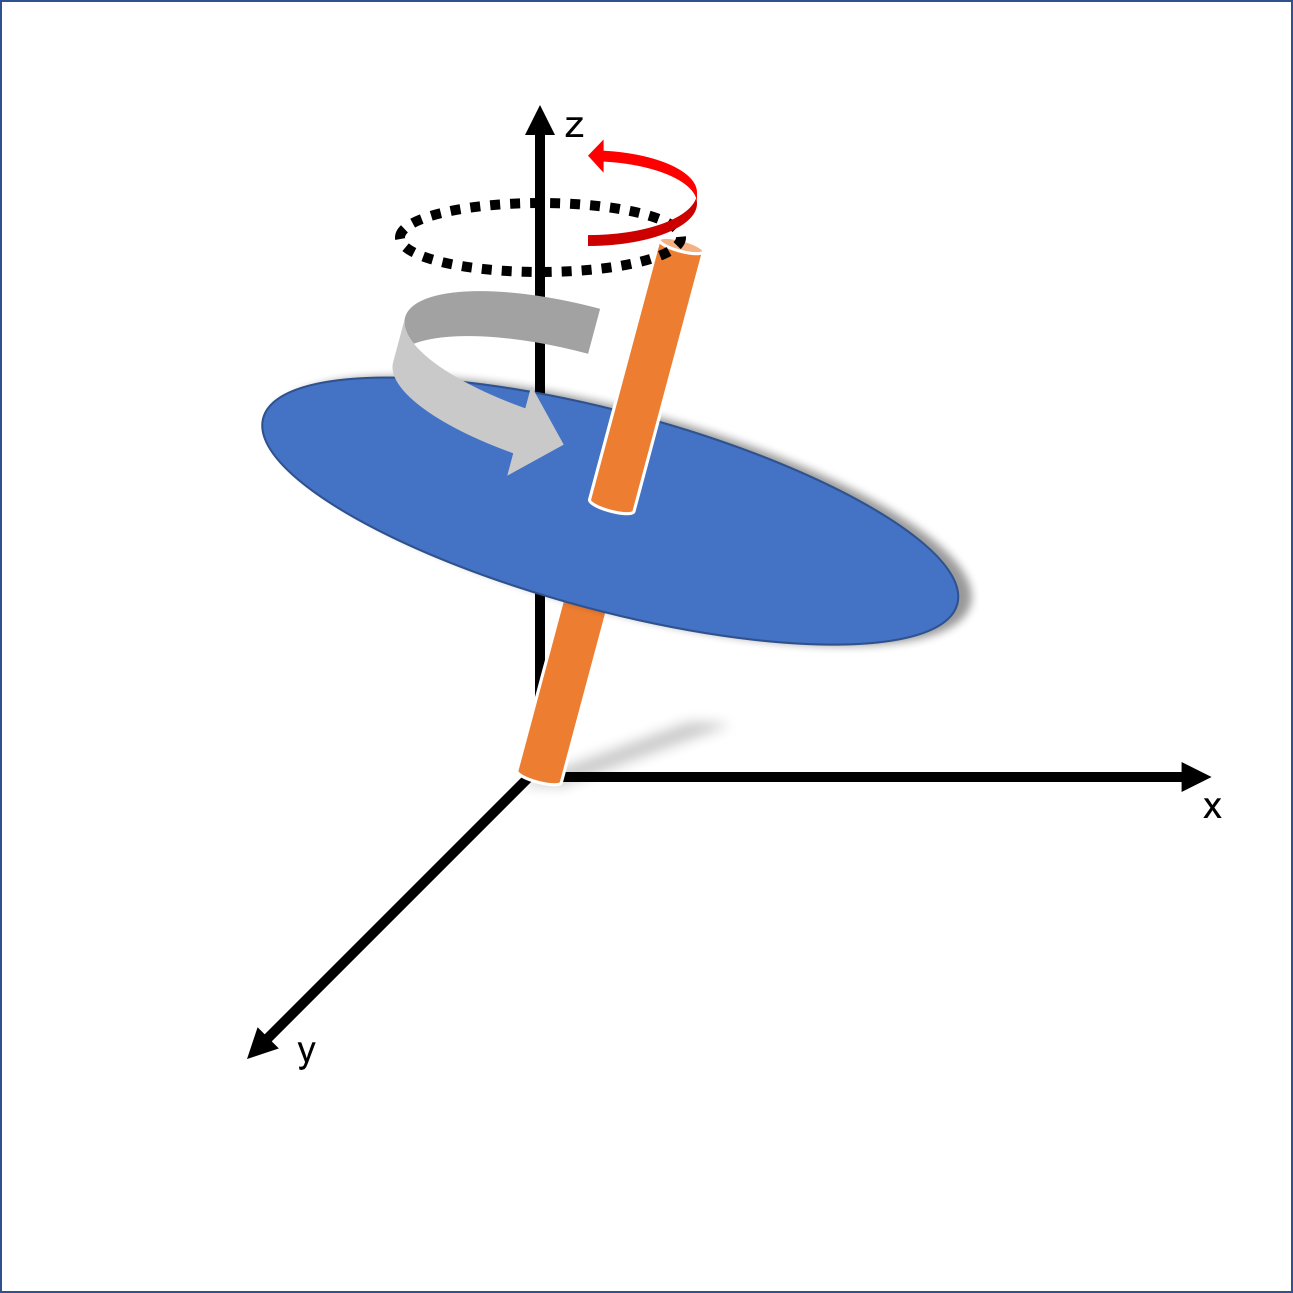
\includegraphics[width=0.8\textwidth]{sphere1.png}
%%	\caption*{\small Figure 2}
\end{figure}

\end{frame}

\begin{frame}{Refinement}

Minimize $E + \sum_{e=1}^{\text{\# of edges}}l_{e}^3$, where $l_{e}$ represents the length of the $e\nth$ edge.

\vspace{5mm}

Limit the possibility that one edge will get extremely long compared to other edges, and therefore limit the possibility that triangles will get deformed.

\vspace{5mm}

This gives us
\begin{equation}
\frac{dX_{k}}{dt} = - \frac{\partial E}{\partial X_{k}} - \frac{\partial \sum_{e} l_{e}^3 }{\partial X_{k}} - \lambda \frac{\partial V}{\partial X_{k}} - \mu \frac{\partial A}{\partial X_{k}}. \nonumber
\end{equation}

%Normal movement: $\frac{dX_{k}}{dt} = N_{k}\cdot S_{k}$; Minimizing $\sum_{f} a_{f}^2$; Constraint local surface areas: Instead of $\frac{dA}{dt} = 0$, we apply $\frac{dA_{local}}{dt} = 0$.
% The advantage of this method is that the squared edge length is related to the elastic potential energy ($E_{elastic} = \frac{1}{2}kx^2$), which resists the deformation of triangles and help to keep the surface smooth.
%did not mention the scale

\end{frame}

\section{Results}

\begin{frame}
\begin{figure}
	\begin{minipage}{0.49\textwidth}
		\centering
		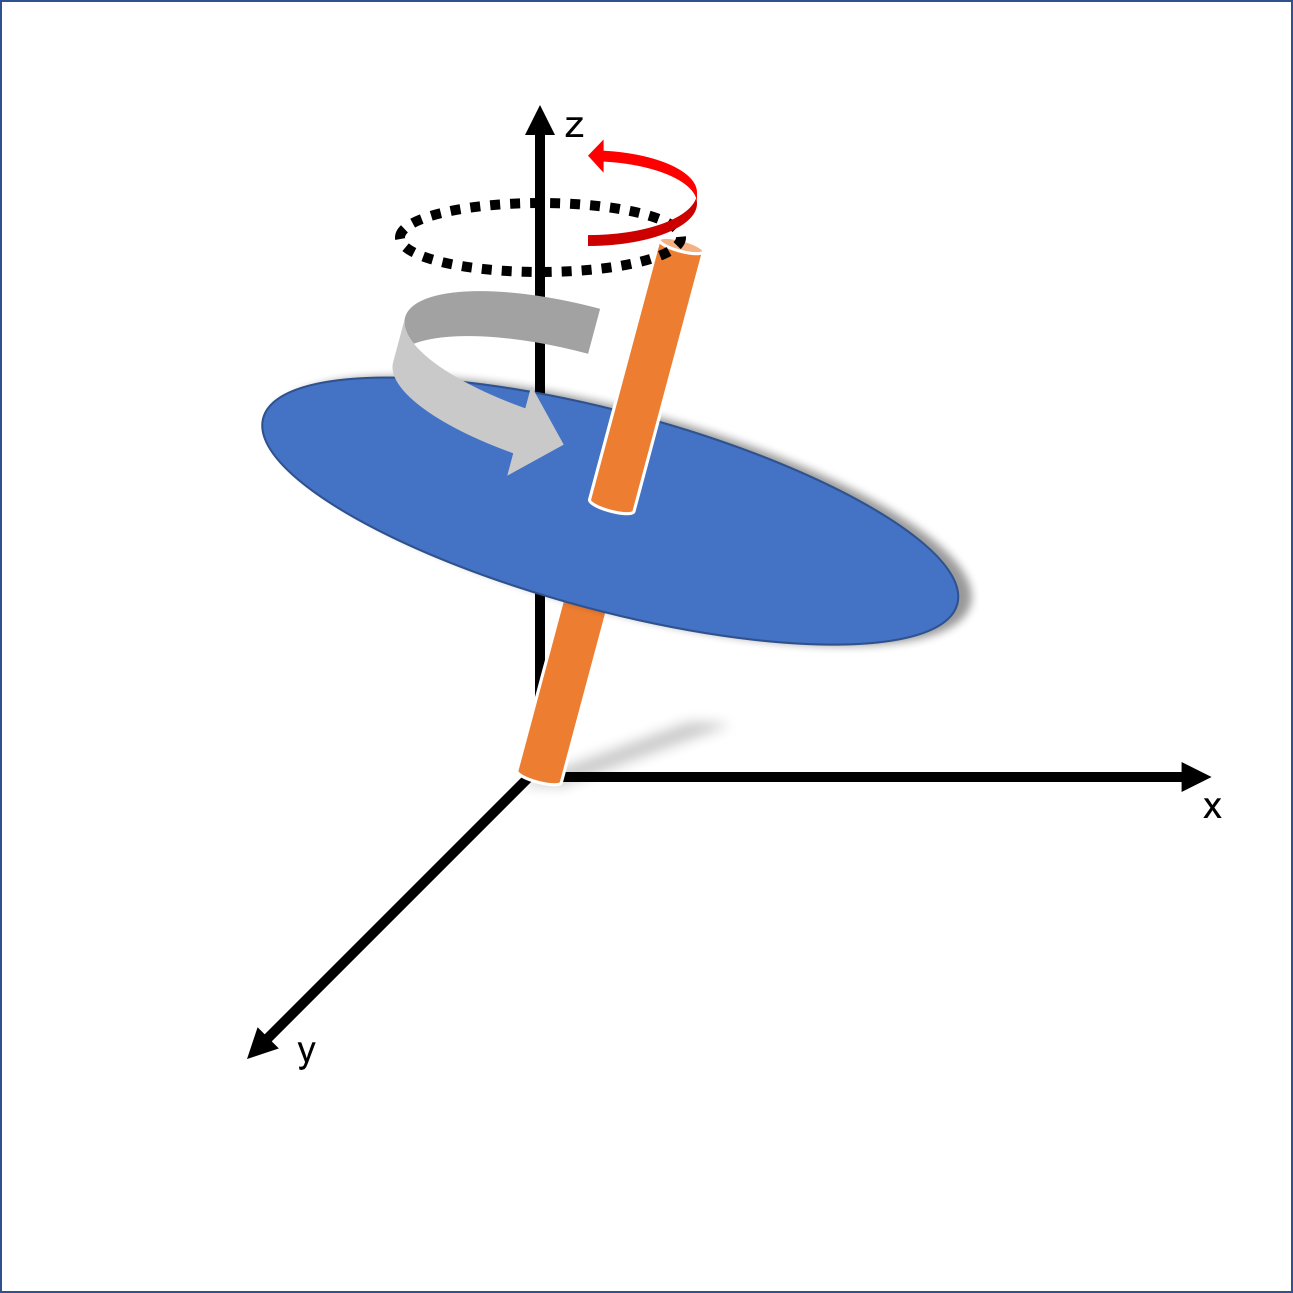
\includegraphics[width=0.85\textwidth]{sphere1.png}
	\end{minipage}
	\begin{minipage}{0.49\textwidth}
		\centering
		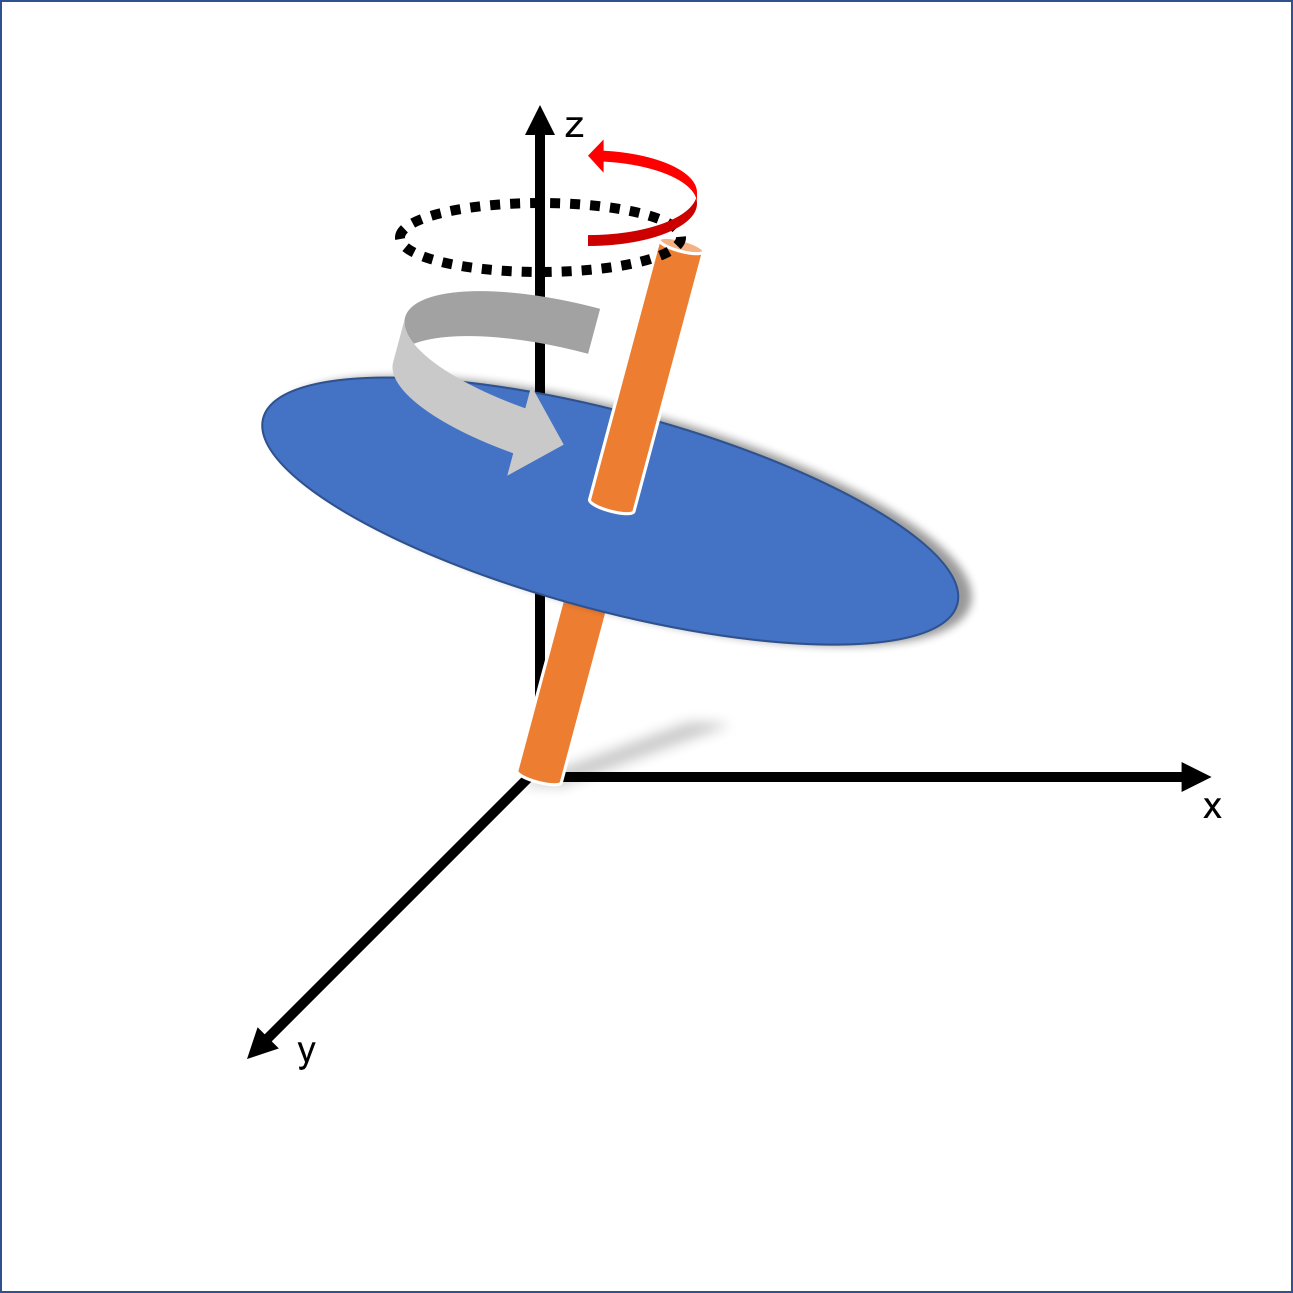
\includegraphics[width=0.85\textwidth]{sphere1.png}
	\end{minipage}

	\begin{minipage}{0.49\textwidth}
		\centering
		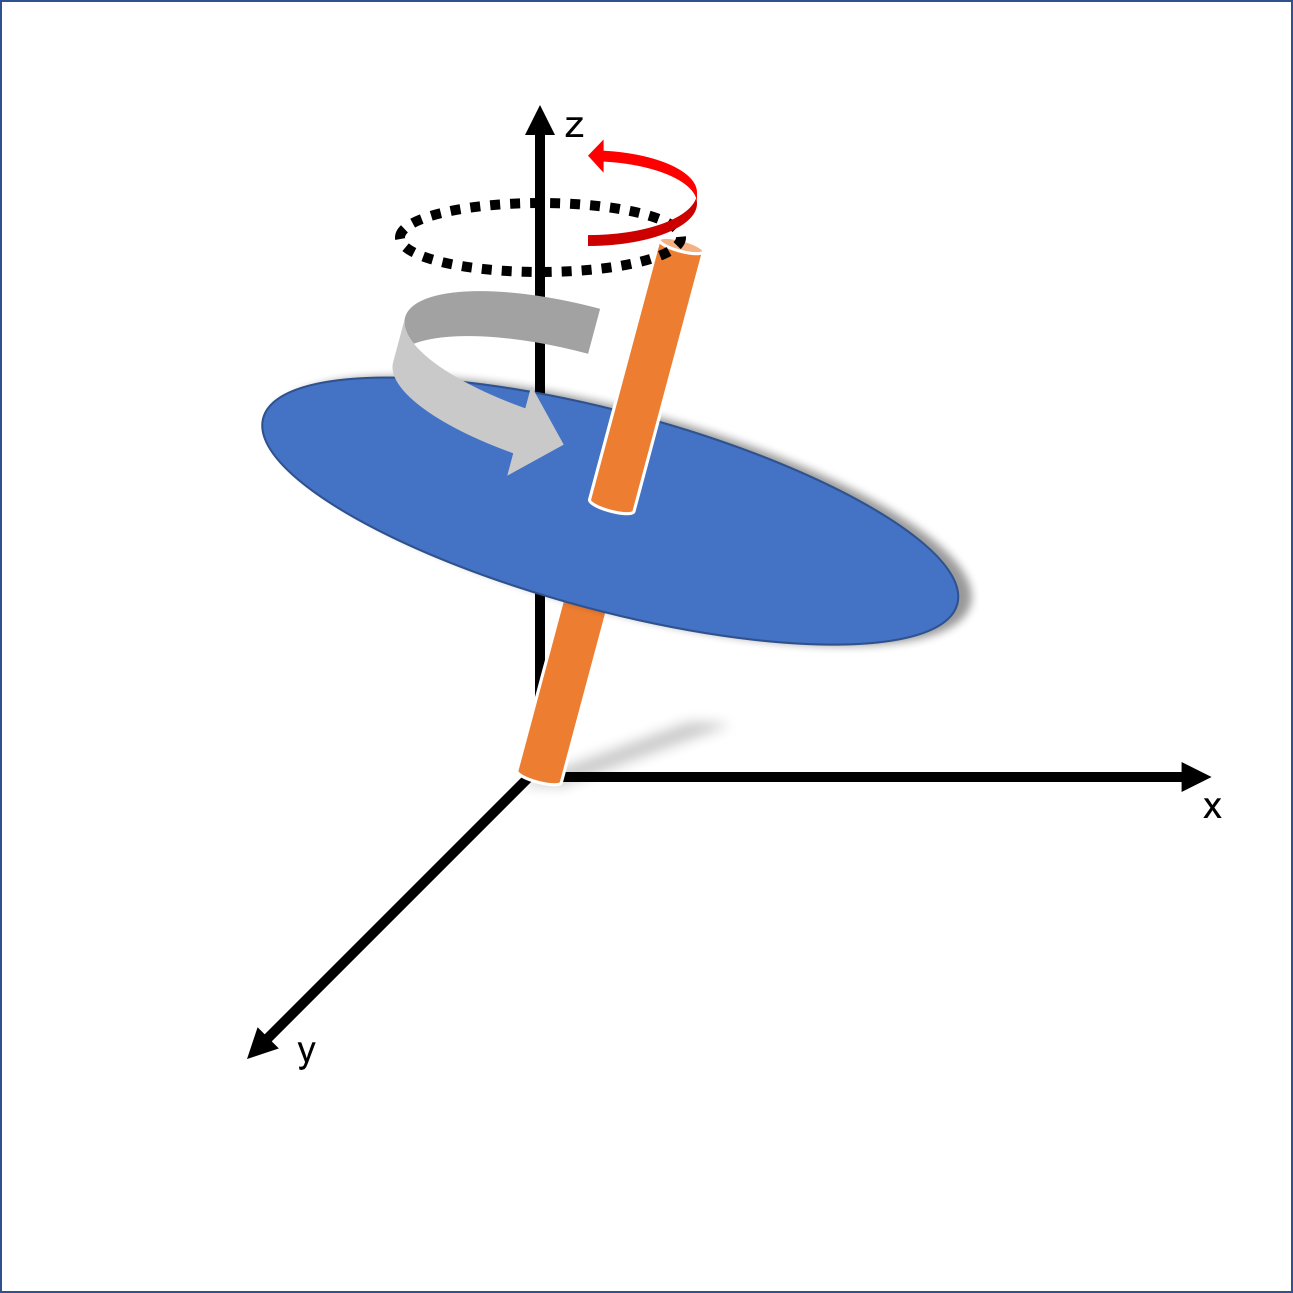
\includegraphics[width=0.9\textwidth]{sphere1.png}
	\end{minipage}
	\begin{minipage}{0.49\textwidth}
		\centering
		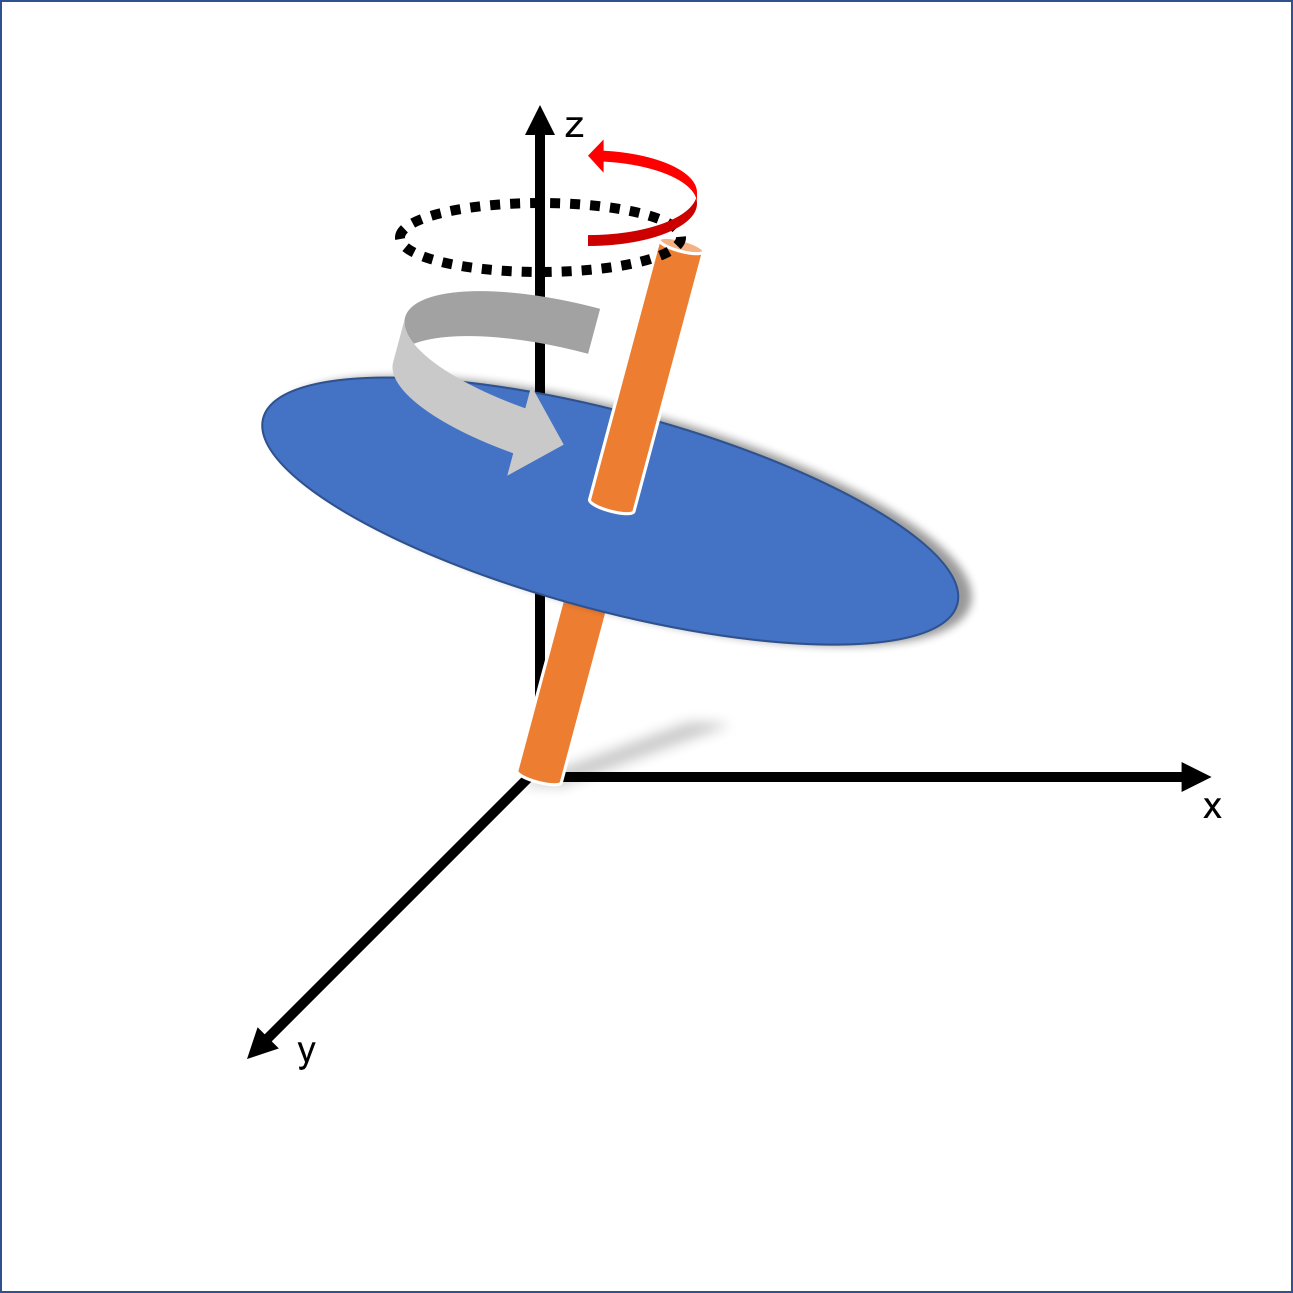
\includegraphics[width=1.0\textwidth]{sphere1.png}
	\end{minipage}

	\begin{minipage}{0.49\textwidth}
		\centering
		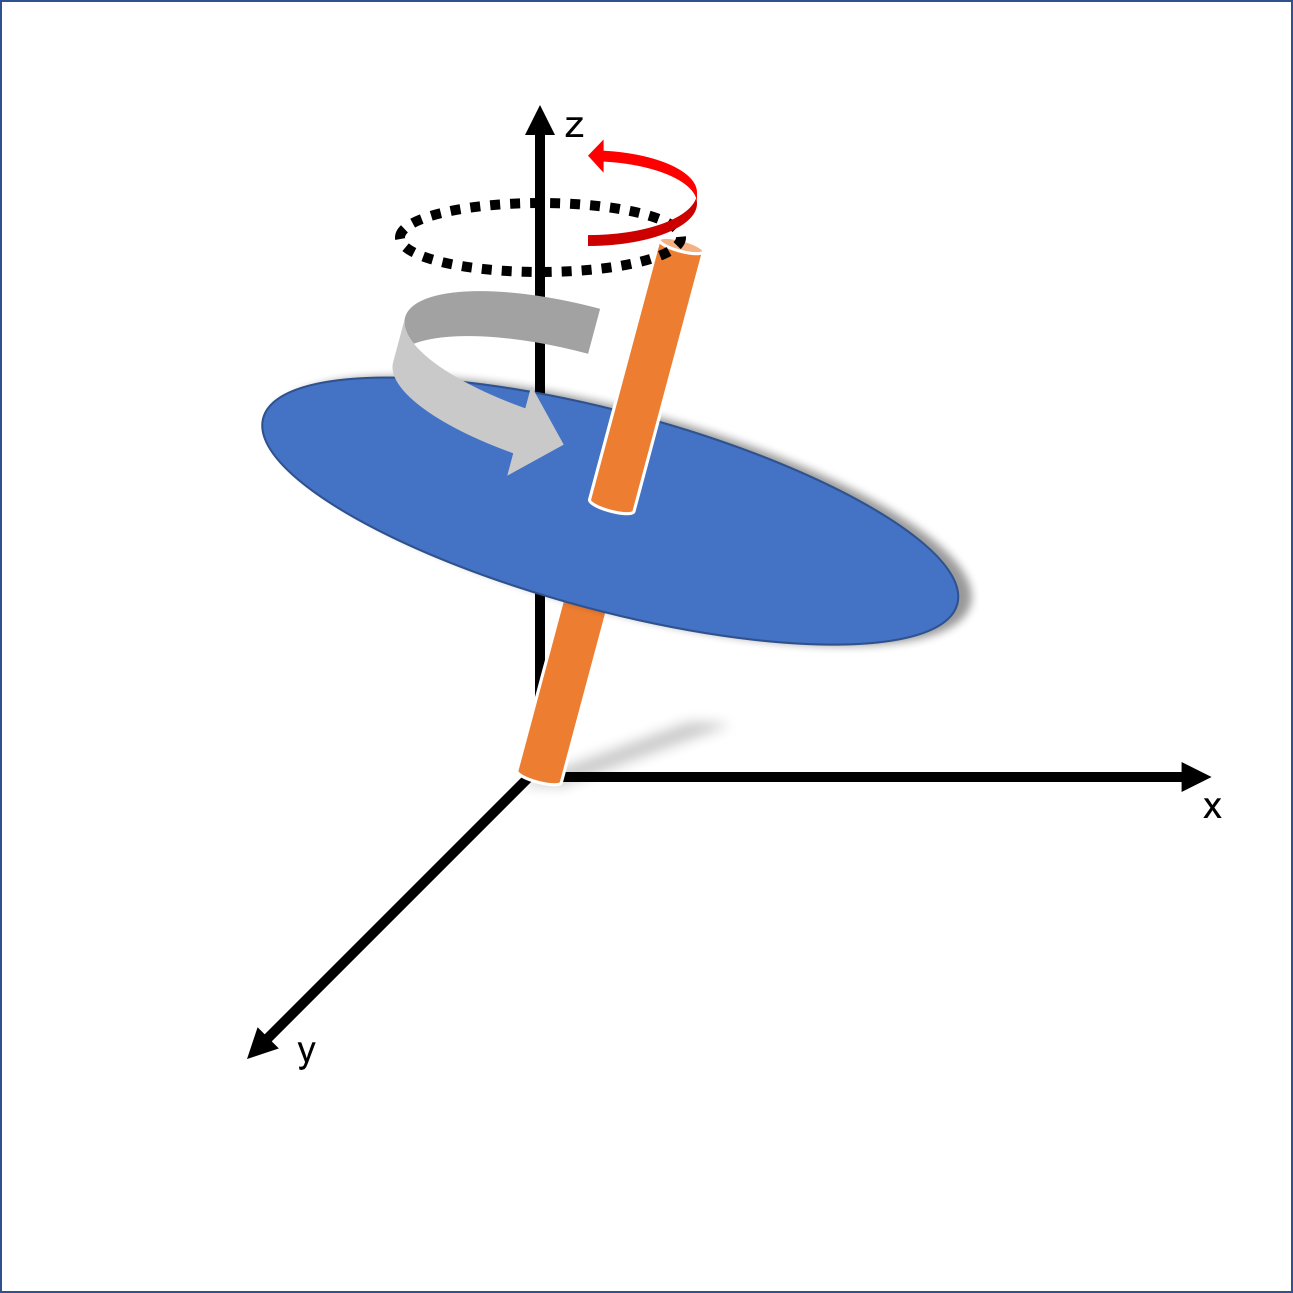
\includegraphics[width=1.0\textwidth]{sphere1.png}
	\end{minipage}
	\begin{minipage}{0.49\textwidth}
		\centering
		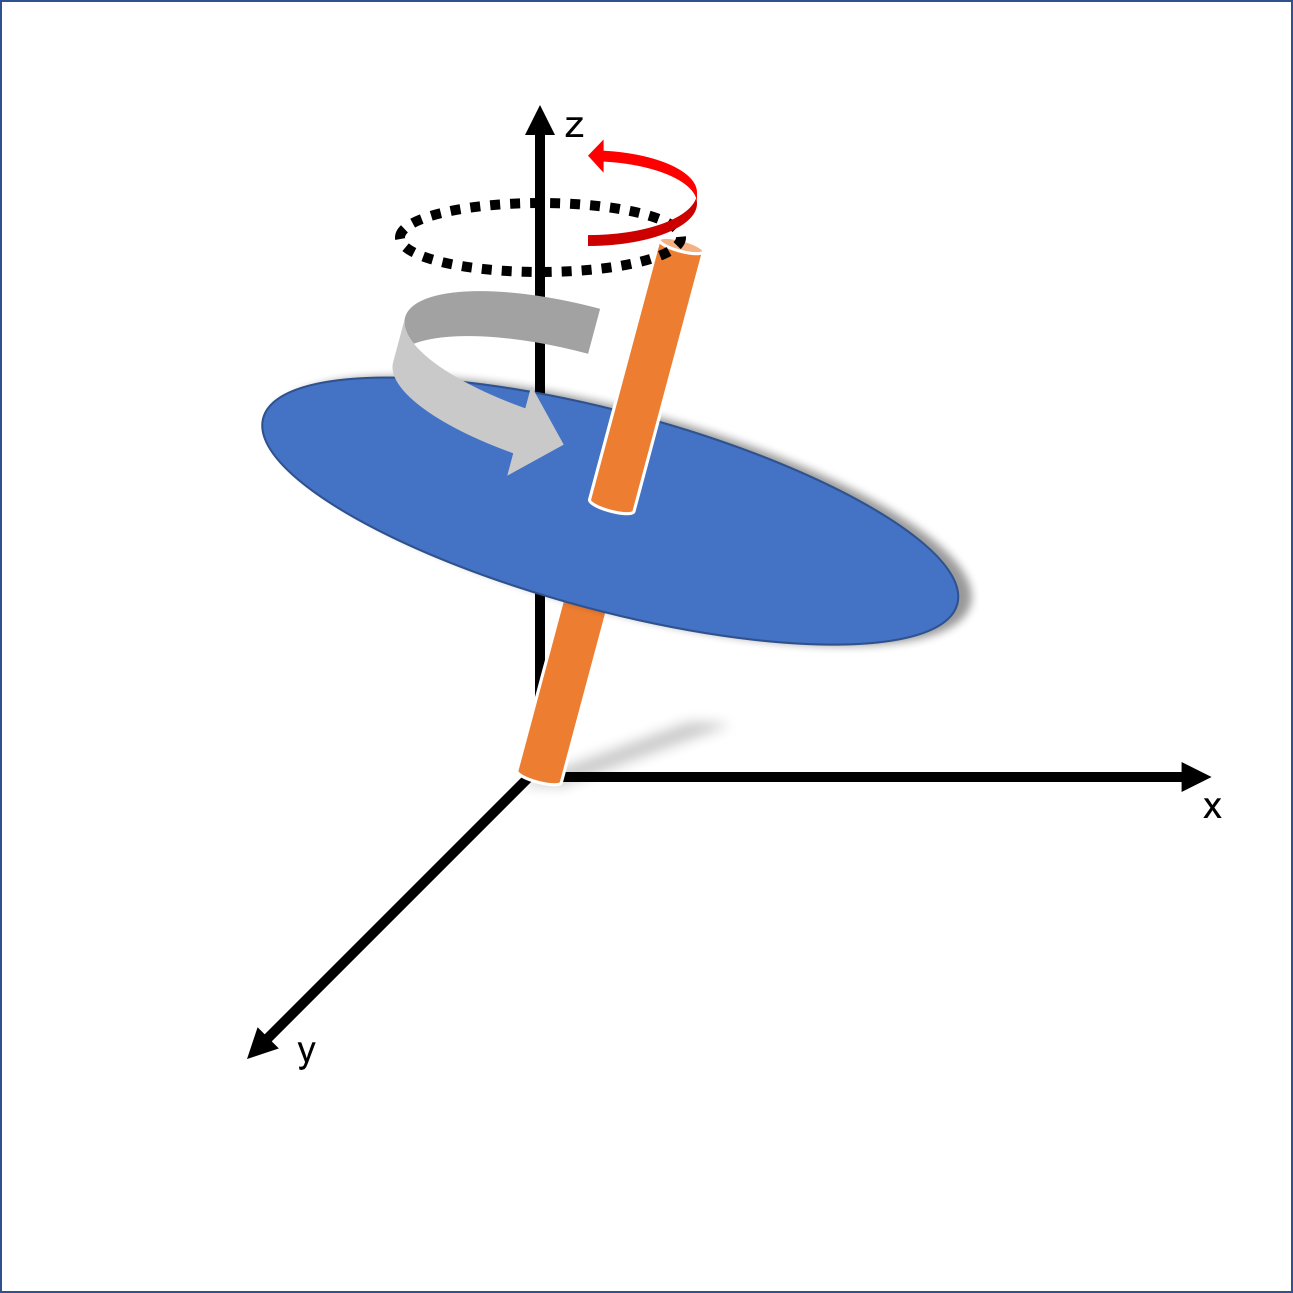
\includegraphics[width=0.9\textwidth]{sphere1.png}
	\end{minipage}


\end{figure}
\end{frame}


\begin{frame}
%Figure 3 shows the result at an early step $t = 0.5$ and figure 4(a) and (b) show the result at $t = 1.8$. From figure 4(b), we can see that the surface is perfectly round viewing from the top, which is exactly how red blood cell looks from the same point of view. However, viewing from the side, as shown in figure 4(a), the upper and bottom surfaces haven't bend inward as expected. Giving the model more time, we have result at $t = 2.3$ as shown in figure 5. Although this figure shows a sign that the upper and bottom surfaces are bending towards inside, the instabilities at the equator are serious problems that need to be fixed.
%add histogram to that these refinement works

%Although the model has not successfully produced a good biconcave, it performs well in following constraints in equations \ref{eq:1}. Figure 6 shows that the total surface area $A$ has not make remarkable change in the time range $[0\text{ }1.8]$, so the constraint on area $\frac{dA}{dt} = 0$ is followed. Figure 7 shows that the total volume $V$ is changing with $V_{0}$ curve in the time range $[0\text{ }1.8]$, so the constraint on volume $\frac{dV}{dt} = \frac{dV_{0}}{dt}$ is followed.


At time t = 1.2,

\begin{figure}[h]
	\begin{minipage}{0.6\textwidth}
		\centering
		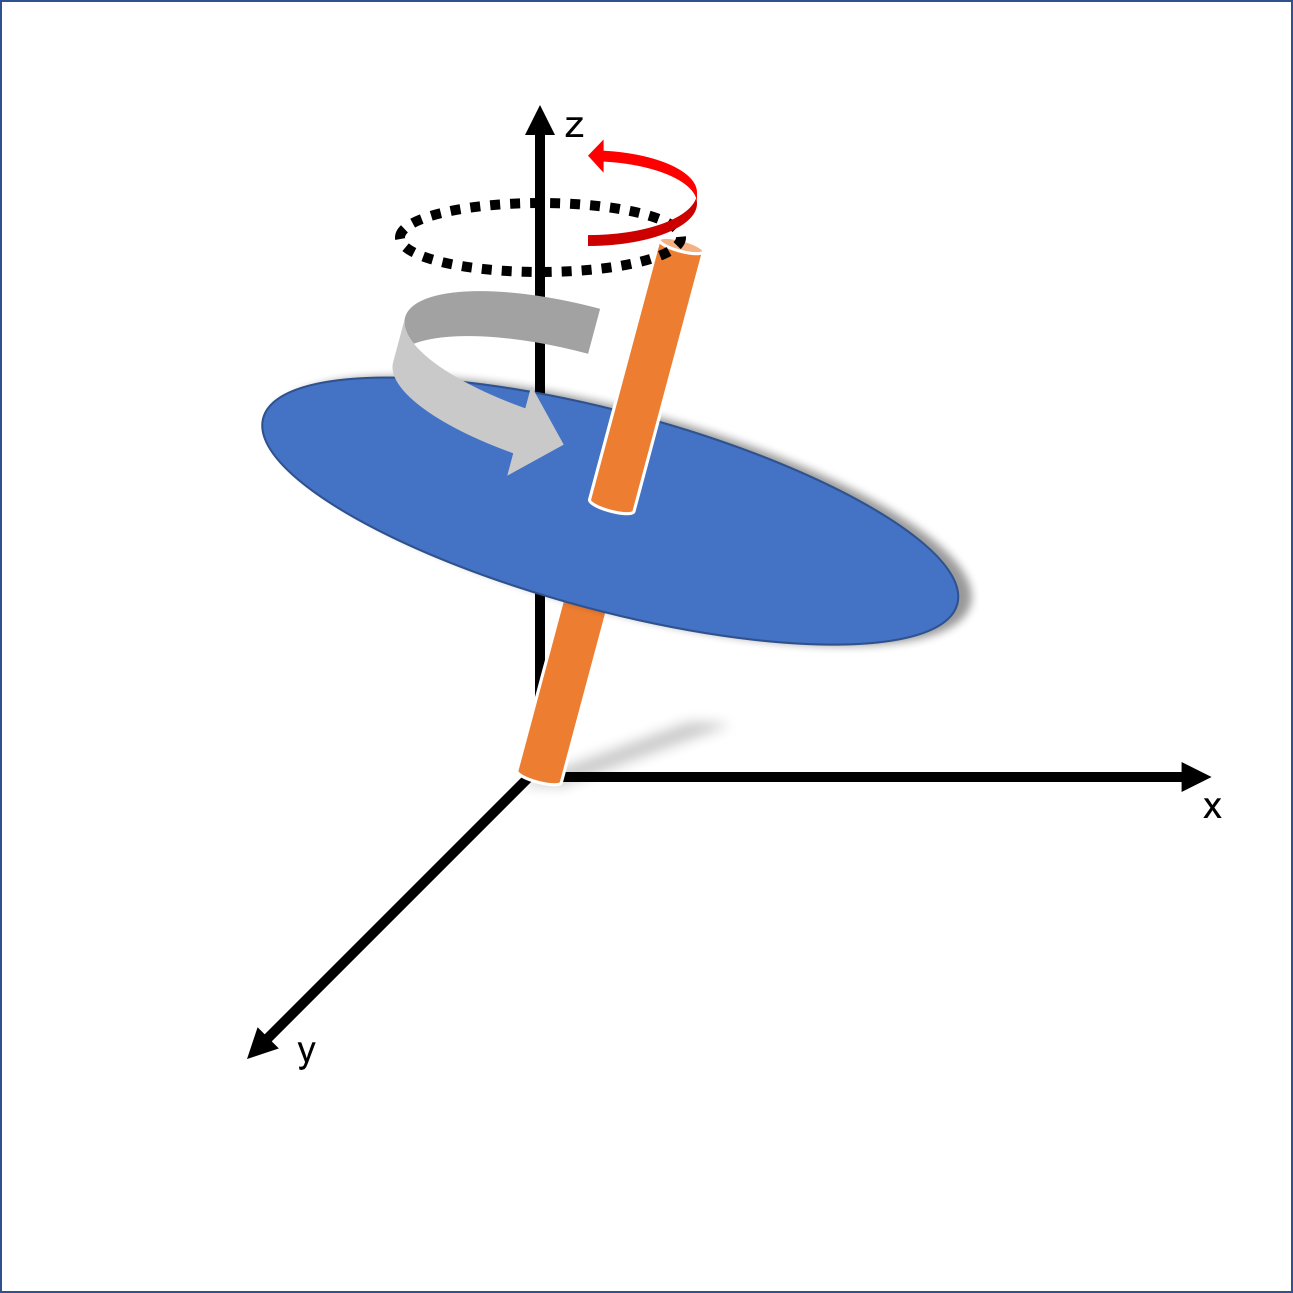
\includegraphics[width=0.9\textwidth]{sphere1.png}
	\end{minipage}

\begin{minipage}{0.45\textwidth}
	\centering
	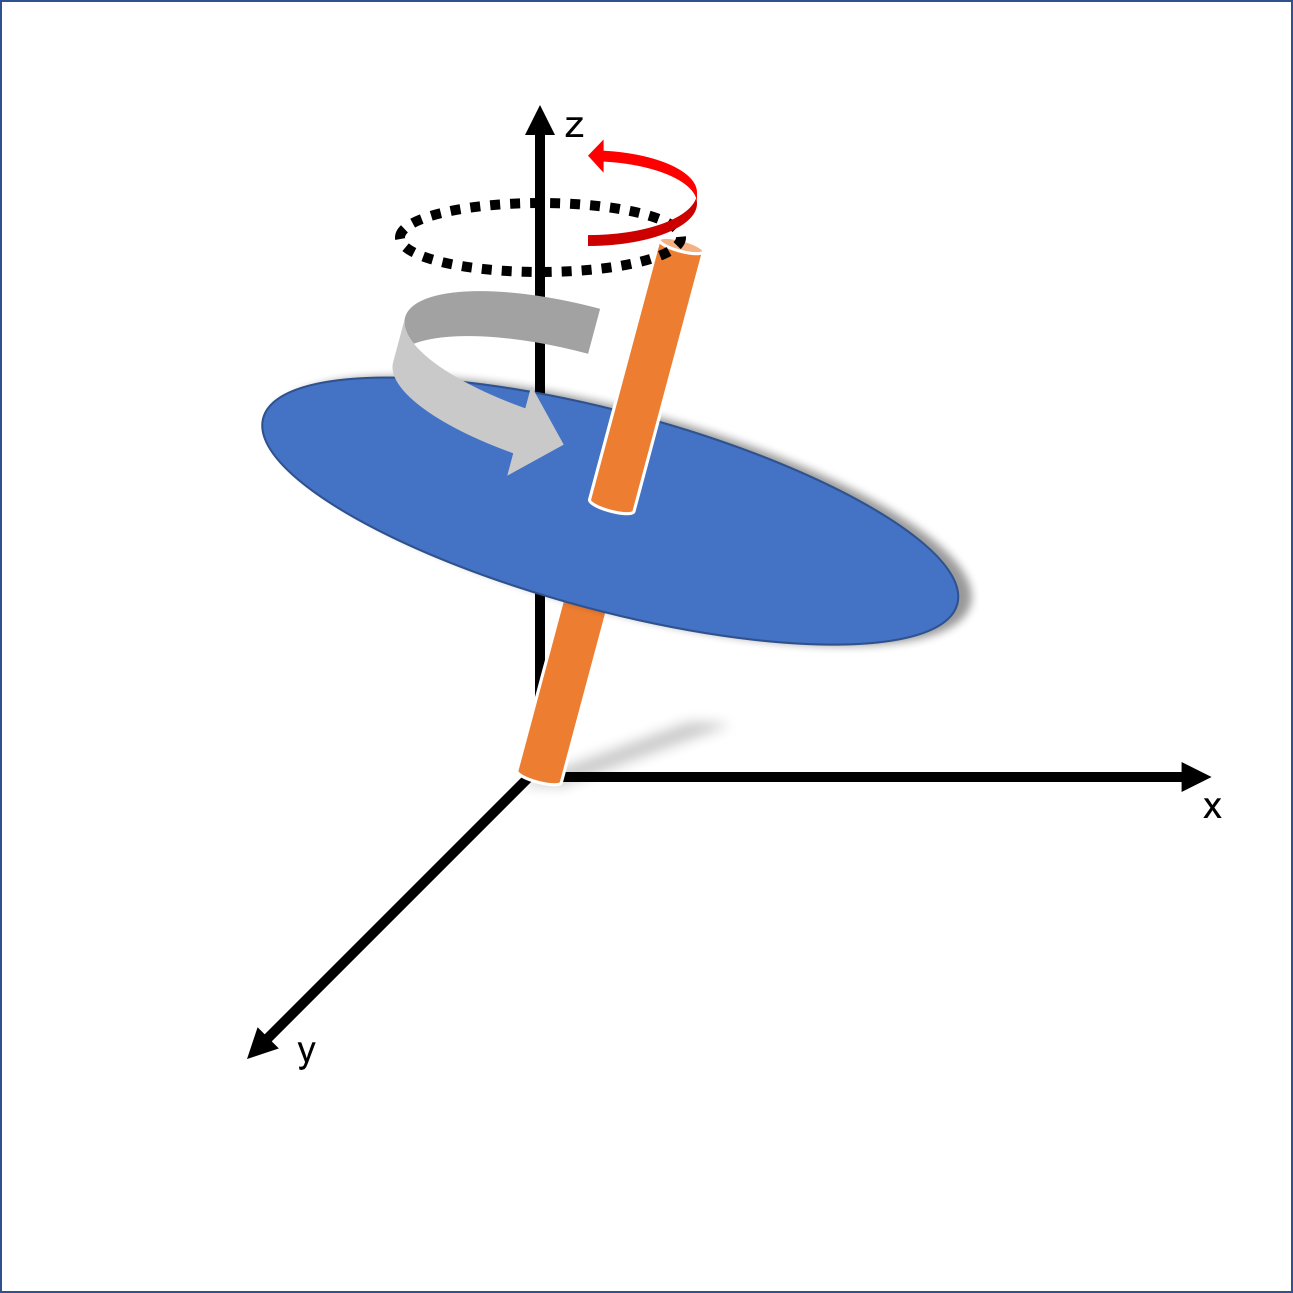
\includegraphics[width=1.1\textwidth]{sphere1.png}
\end{minipage}
	\begin{minipage}{0.45\textwidth}
		\centering
		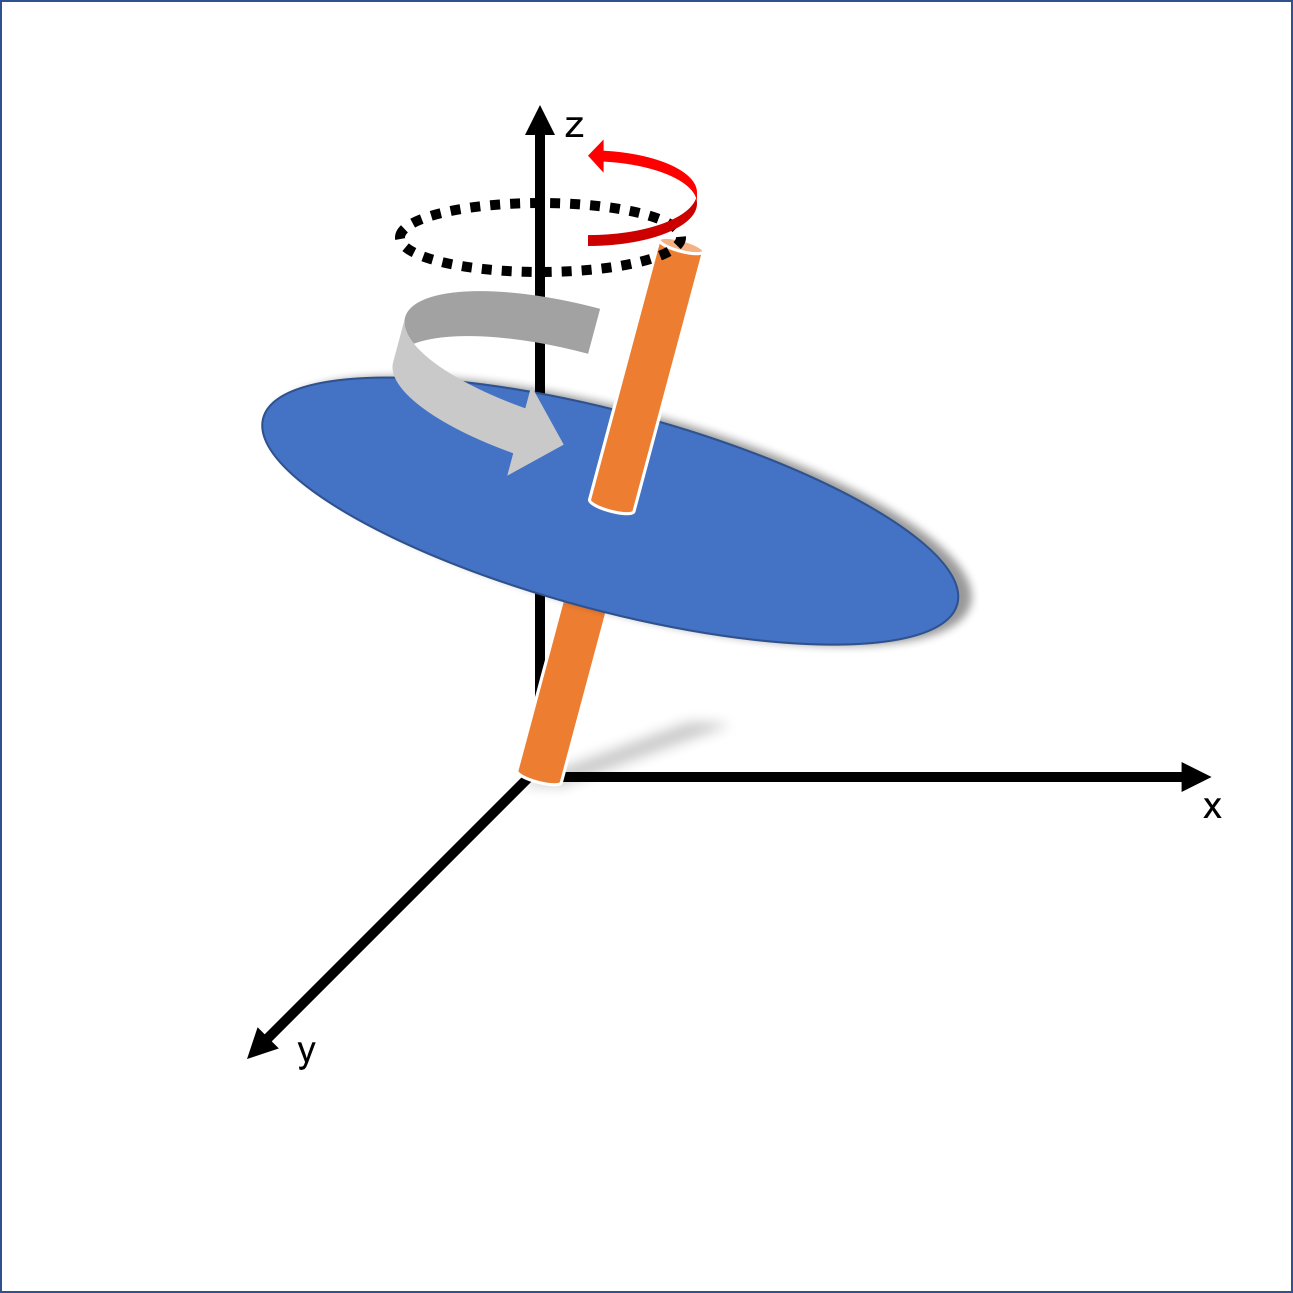
\includegraphics[width=0.9\textwidth]{sphere1.png}
	\end{minipage}
\end{figure}

\end{frame}

\begin{frame}

%\begin{center}%
%	\includemovie{.85\textheight}{.85\textheight}{RBC-3.mov}%
%\end{center}%

\end{frame}

\begin{figure}[h]
	\begin{minipage}{0.6\textwidth}
		\centering
		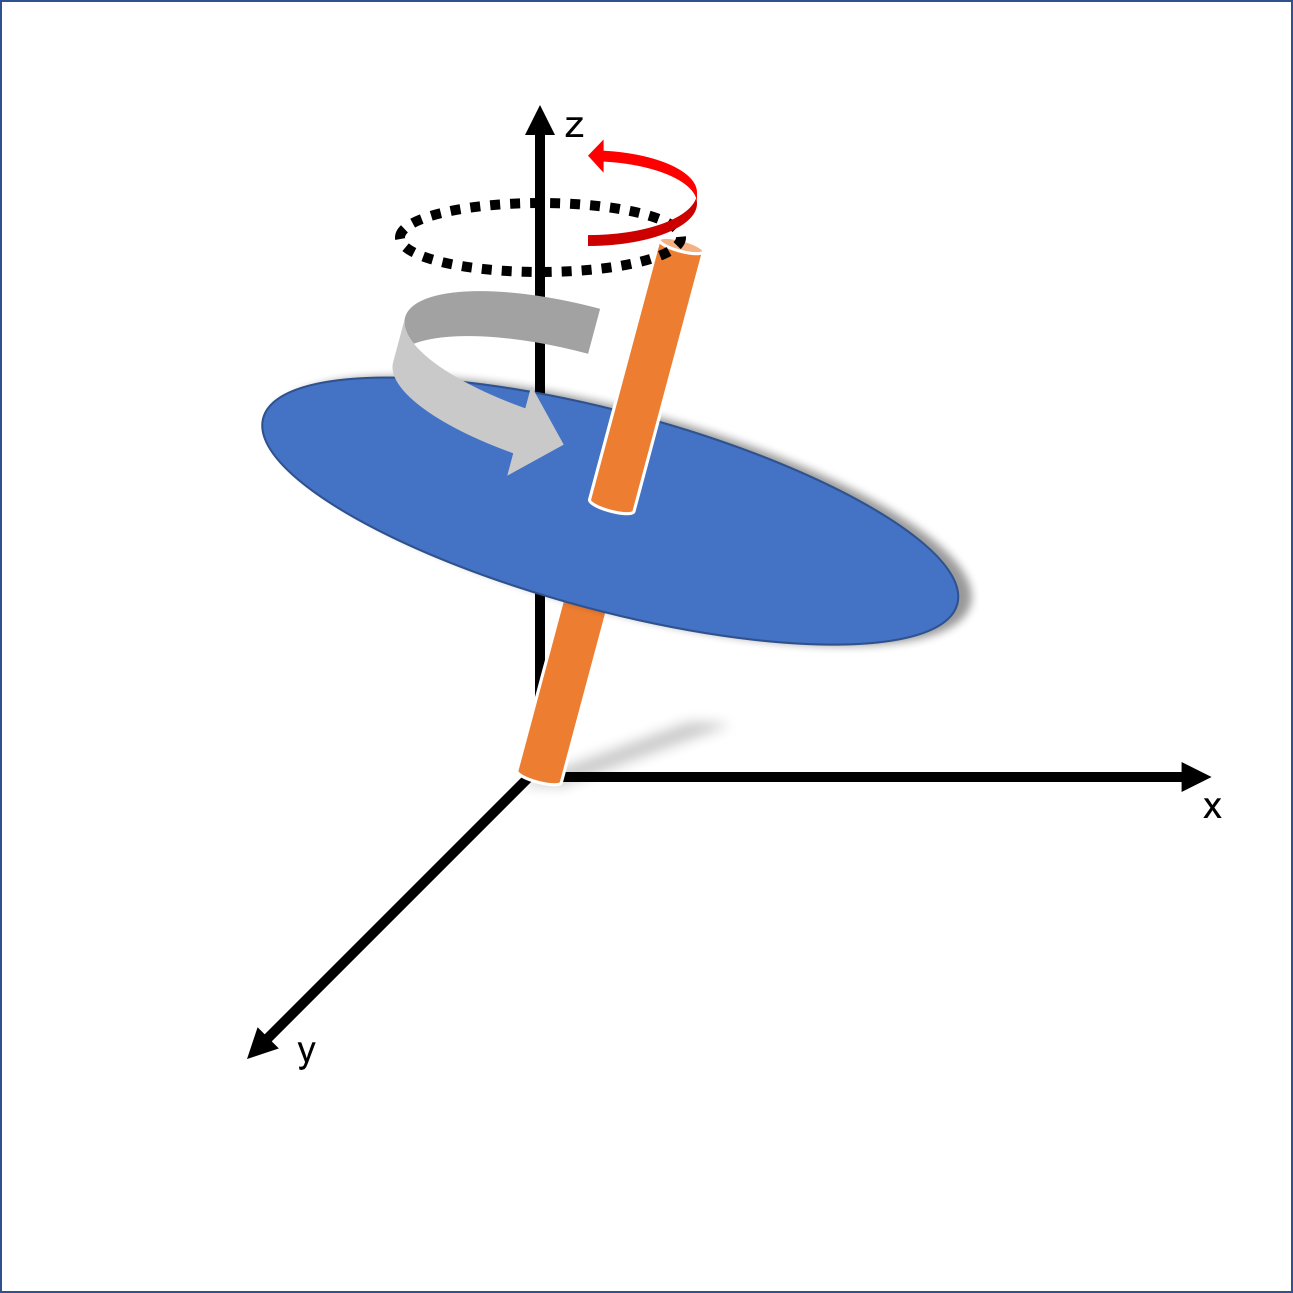
\includegraphics[width=0.95\textwidth]{sphere1.png}
	\end{minipage}

	\begin{minipage}{0.6\textwidth}
		\centering
		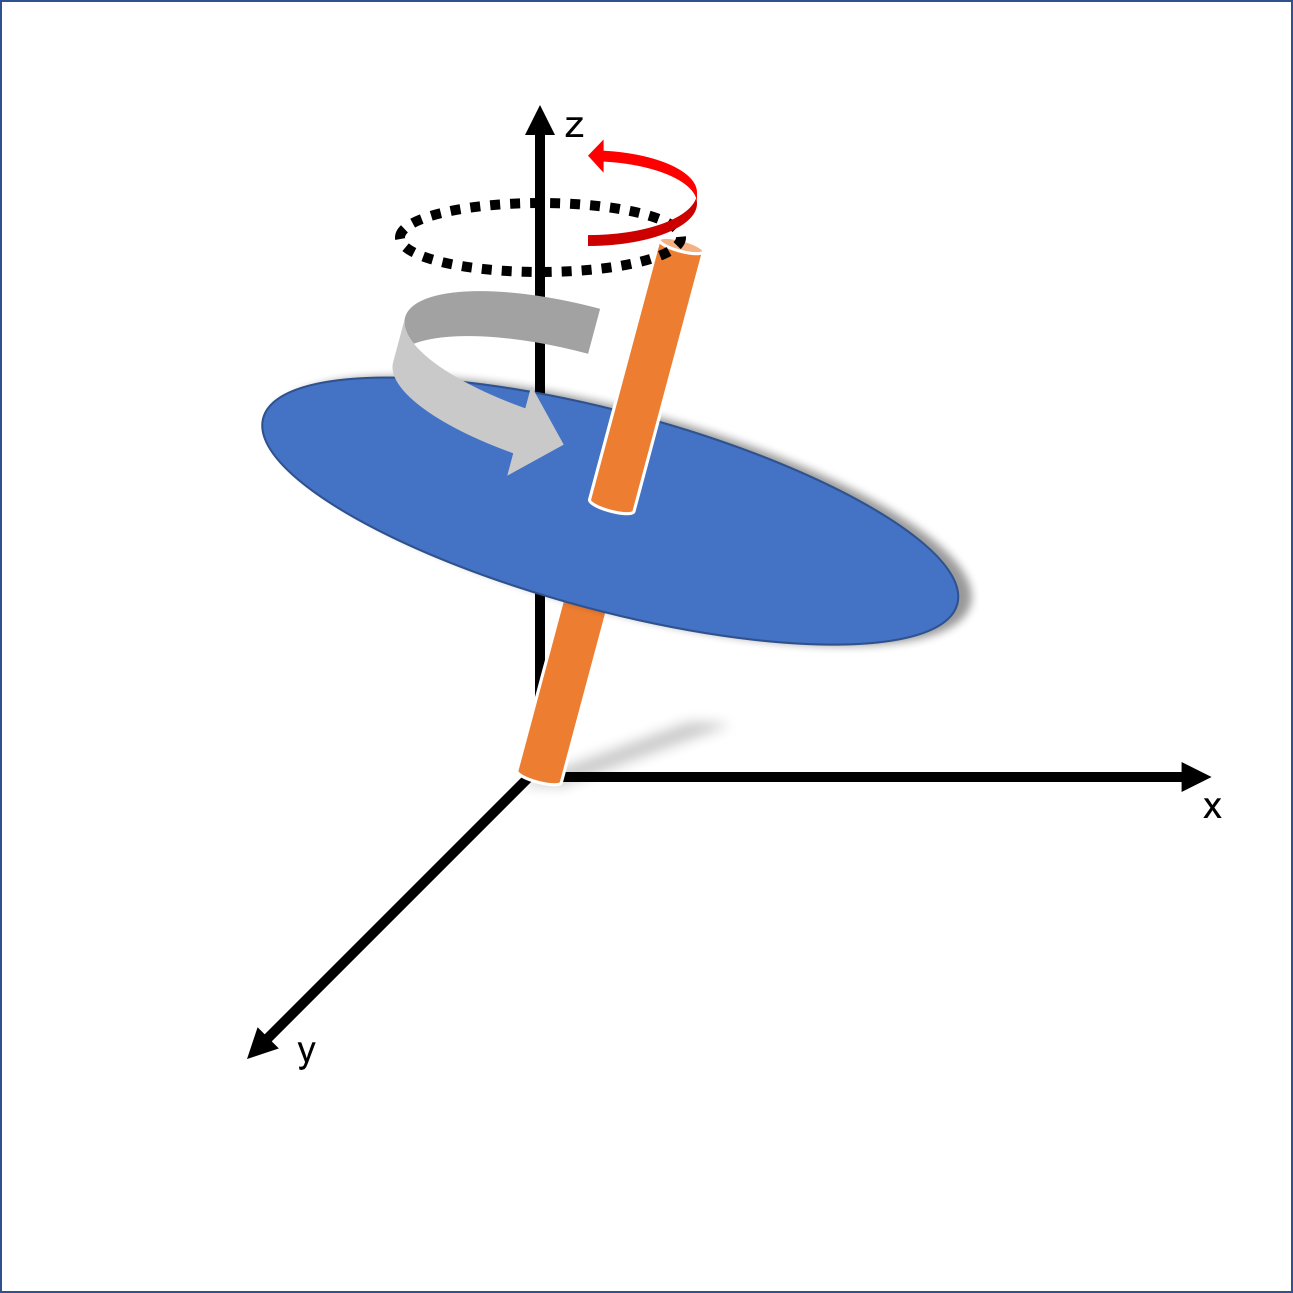
\includegraphics[width=0.70\textwidth]{sphere1.png}
	\end{minipage}
\end{figure}


\begin{frame}
\begin{figure}
	\centering
	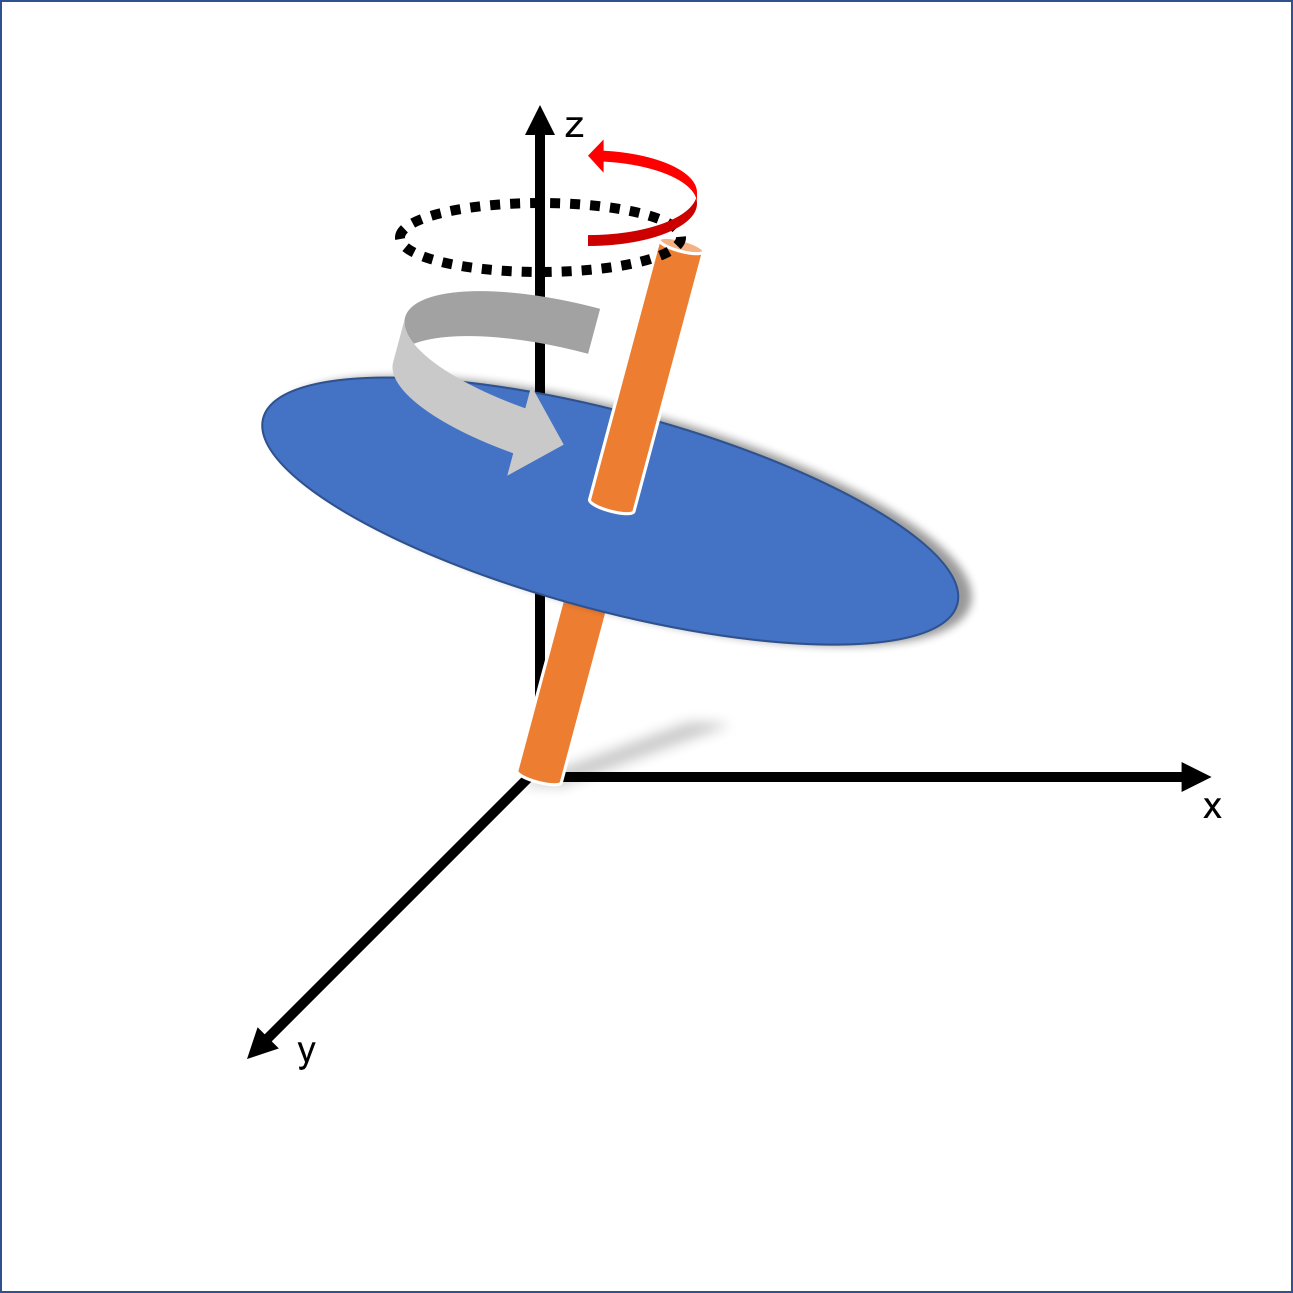
\includegraphics[width=0.87\textwidth]{sphere1.png}

	\vspace{5mm}
	\emph{Constraint: $\frac{dA}{dt} = 0$.}
\end{figure}
\end{frame}

\begin{frame}
\begin{figure}
	\centering
	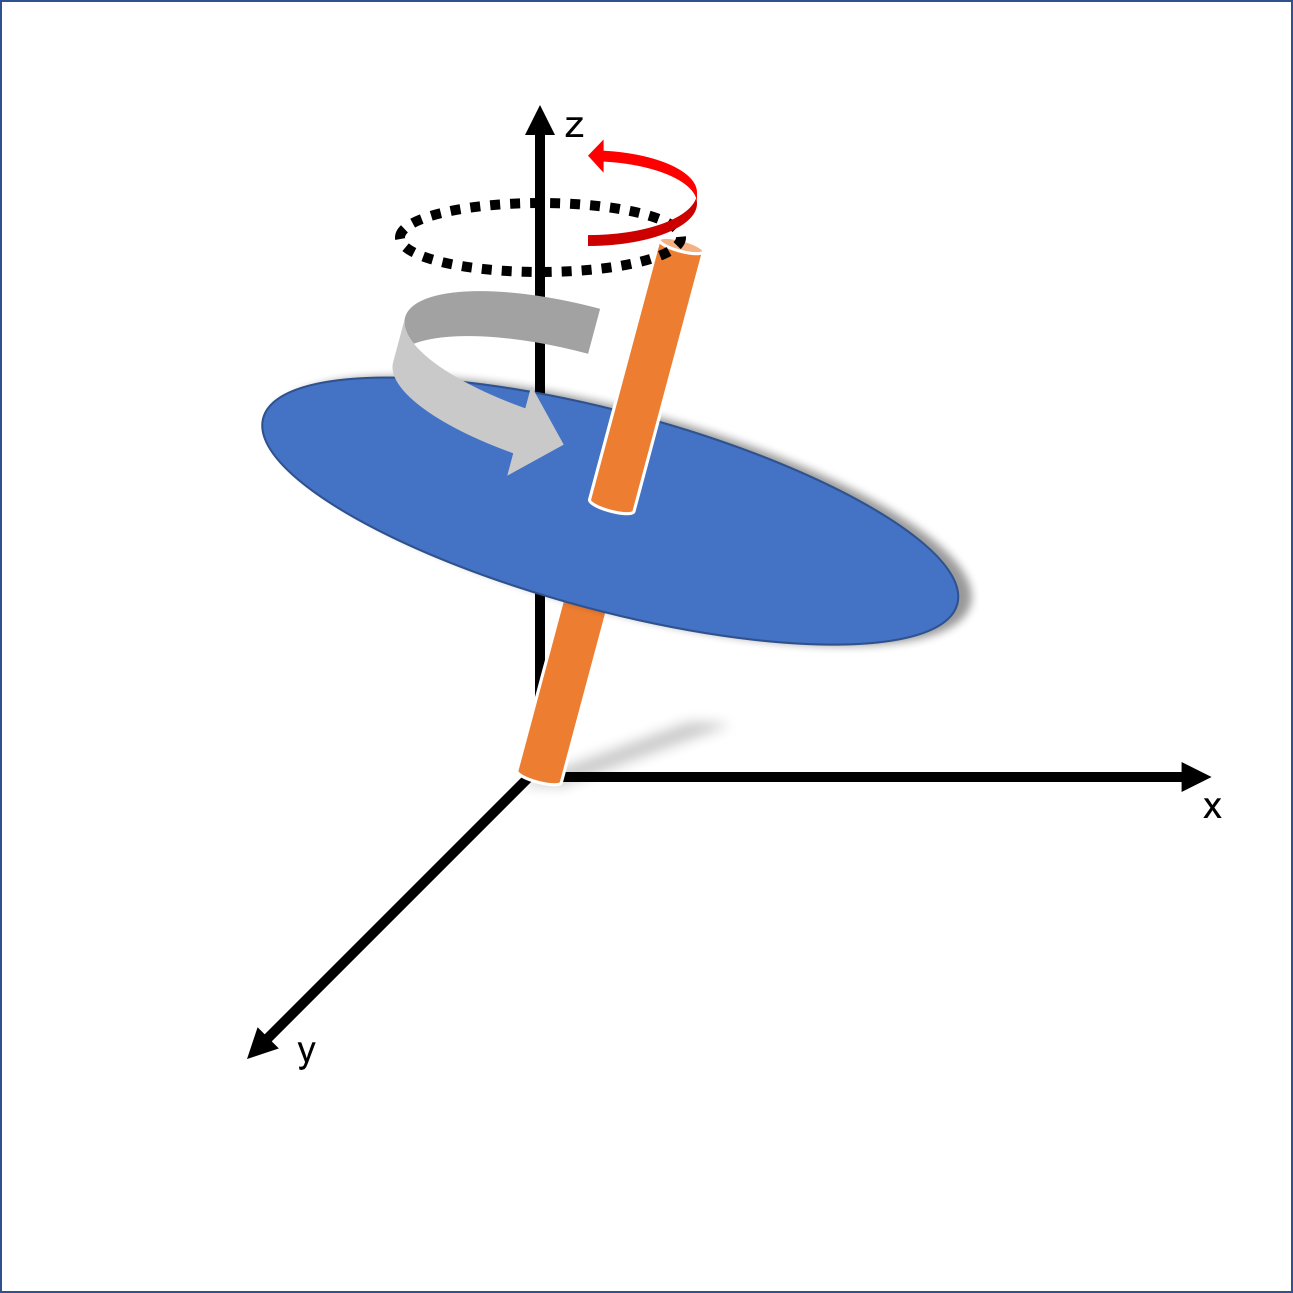
\includegraphics[width=0.87\textwidth]{sphere1.png}

	\vspace{5mm}
	\emph{Constraint: $\frac{dV}{dt} = \frac{dV_{0}}{dt}$, where $V_{0}(t) = V\min + (V\max-V\min)e^{-at}$.}
\end{figure}

\end{frame}


\section{Conclusion}

\begin{frame}

(1) Generate a shape that is close to biconcave, but not exactly the same.

(2) Possible explanations for the instabilities.

(3) Look into the future.

\end{frame}


\begin{figure}[h]
	\begin{minipage}{0.6\textwidth}
		\centering
		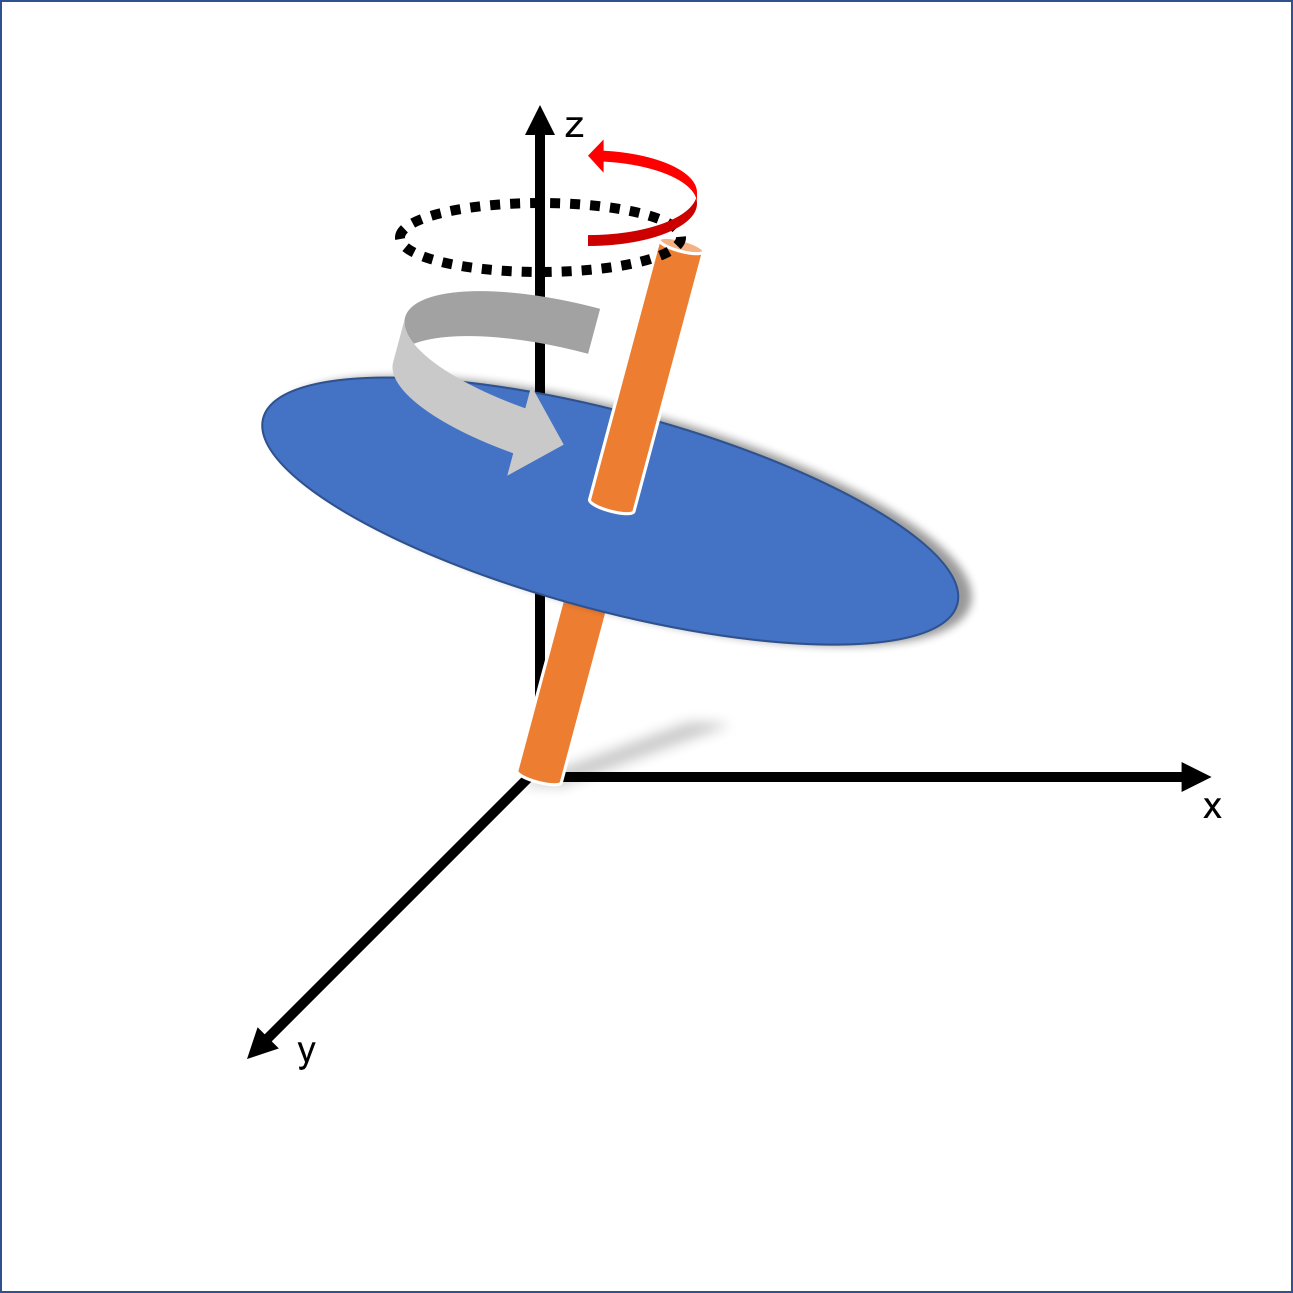
\includegraphics[width=0.7\textwidth]{sphere1.png}
	\end{minipage}
	\begin{minipage}{0.6\textwidth}
		\centering
		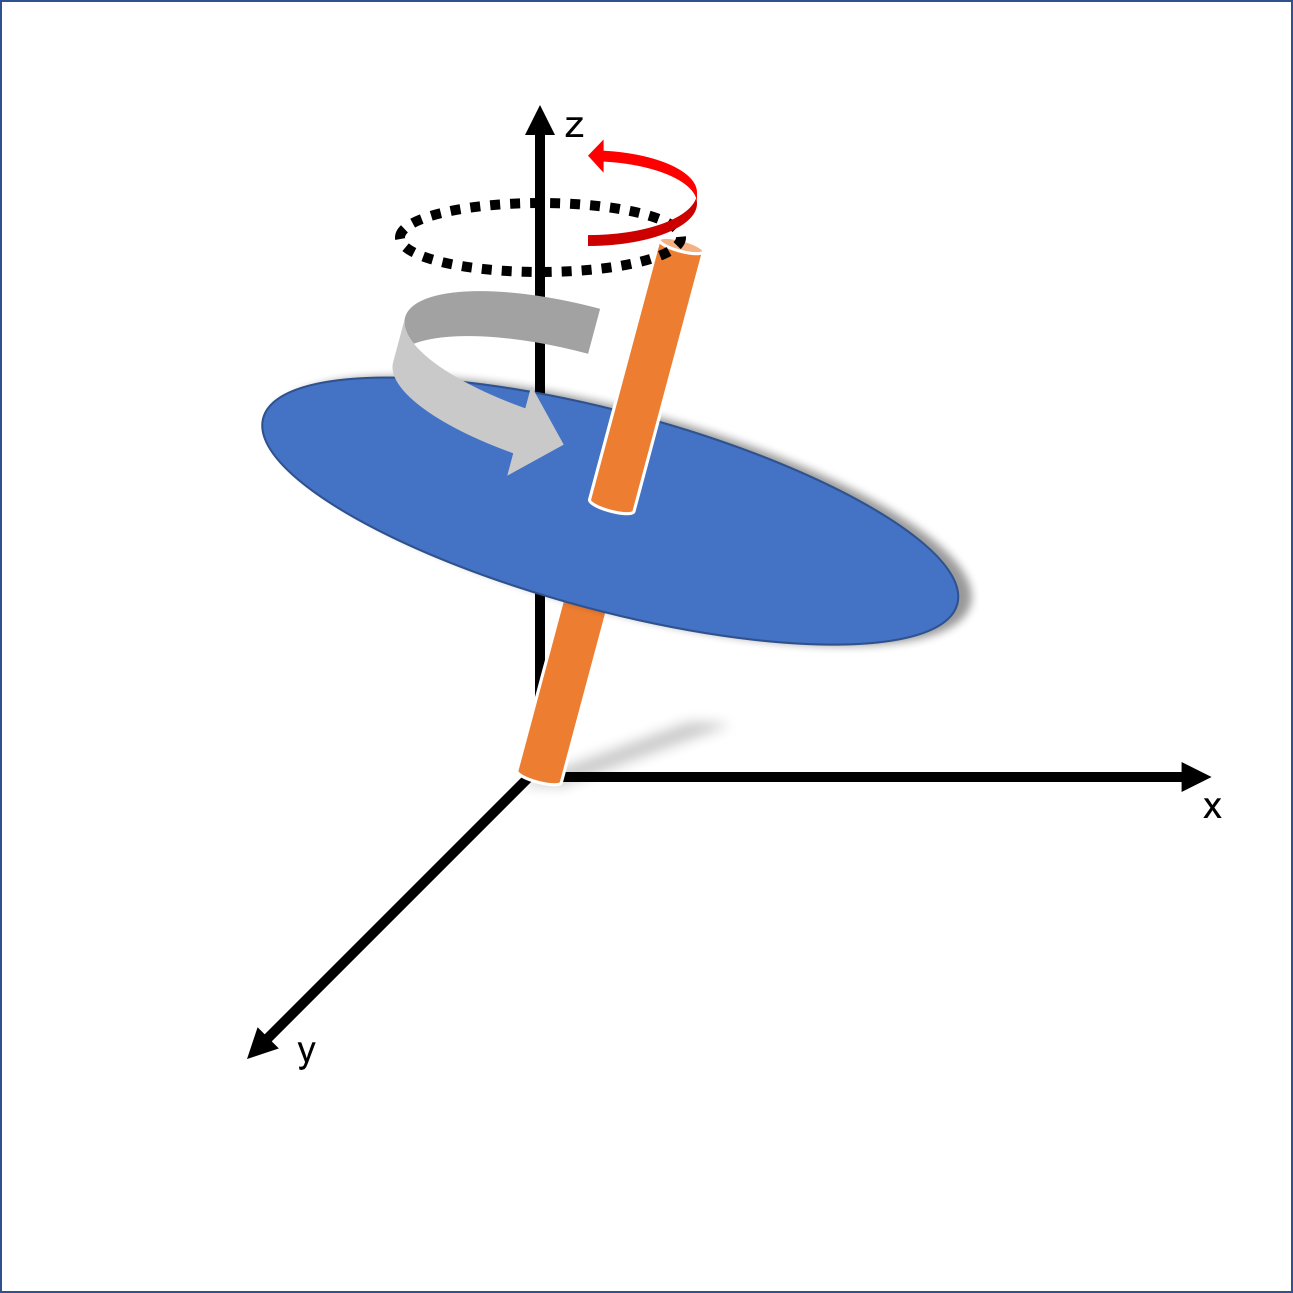
\includegraphics[width=0.7\textwidth]{sphere1.png}
	\end{minipage}
\end{figure}


\begin{frame}{Acknowledgement}

 I would like to show my gratitude to my mentor Professor Charles S. Peskin for his great guidance and encouragement. It is his wisdom that shows me the light through difficulties.

 I would also like to present my special thanks to Dr. Pejman Sanaei and Mr. Jason Kaye for their patient assitance and critiques of the research project.

 I would also like to thank Professors Miranda Holmes-Cerfon and Aleksandar Donev for leading and supporting the undergraduate research program.

 Finally, I would like to thank NYU Math Department for funding this research.

\end{frame}

\begin{frame}{Reference}
\begin{thebibliography}{9}
	\bibitem{Reece}
	Reece, J. B., Urry, L. A., Cain, M. L. 1., Wasserman, S. A., Minorsky, P. V., Jackson, R., and Campbell, N. A. (2014).
	\textit{Campbell biology.} Tenth edition.
	Boston: Pearson.

	\bibitem{sphere}
	Charles S. Peskin.
	Matlab codes that generate a sphere.

	\bibitem{bendingE}
	Charles S. Peskin.
	Notes on defining bending energy on a discrete surface.

	\bibitem{Canham70}
	Canham, P.B. (1970).
	The minimum energy of bending as a possible explanation of the biconcave shape of the human red blood cell.
	\textit{Journal of Theoretical Biology,}
	26(1), 61-81. doi:10.1016/s0022-5193(70)80032-7.

	\bibitem{Sullivan}
	Sullivan, J.M. (2006).
	Curvatures of Smooth and Discrete Surfaces.
	\textit{Discrete Differential Geometry Oberwolfach Seminars,}
	175-188. doi:10.1007/978-3-7643-8621-4\underline{ }9.

\end{thebibliography}

\end{frame}

\end{document}
